\chapter{偏微分方程的数值求解}
\label{chap:pde-numerical-methods}

考虑区间上的边值问题：$-u''=\pi^2\sin(\pi x)$，$u(0)=0$，$u(1)=1$。它的解$u=\sin(\pi x)+x$可以直接写出，所以我们能核对任何近似。换成系数跳变的杆、形状不规则的板，或者会出现激波的车流，解就写不出来了。前面各章告诉我们解是否存在、属于什么空间、信息怎样传播，却没有告诉我们某一点的数值。

计算机只能保存有限个数，把一个场换成有限个数有不同的办法：记录格点上的值，记录一组基函数的系数，或者记录每个小单元里的平均量。这三种记录方式分别对应有限差分、Galerkin有限元和守恒有限体积方法，它们保留的是连续问题的三种不同结构：局部导数、弱形式和局部守恒。

得到一组数之后，真正难的问题才开始：这组数代表了什么？网格加密时它是否趋于原问题的解，趋于哪一个解？第~\ref{chap:scalar-conservation-laws}章已经看到，守恒律的弱解可以不唯一，一个看上去合理的格式完全可能收敛到错误的解。

本章先用上面的区间问题说明三类未知量和误差的三个来源，再依次讲三种方法，每种方法都结合能手算的小网格写出计算过程。随后讨论一致性、稳定性与收敛的关系，线性和非线性问题在这里要走不同的路。最后把空间、时间、积分和代数误差分开检验，并比较计算成本。

本章的结论都在有限时间区间上讨论，长时间行为不在这里考虑；除特别说明外，线性格式的结论针对规则网格。

\section{离散问题}
\label{sec:pdenum-discrete}

一个定义在区间上的函数有无穷多个值，怎样只用有限个数把它留下来？答案不止一种，不同的答案决定了后面的方程长什么样。全章的第一个例子是
\begin{equation}
 -u''=\pi^2\sin(\pi x)\quad\text{于}\ (0,1),\qquad u(0)=0,\quad u(1)=1,
 \label{eq:pdenum-model}
\end{equation}
它的解是
\begin{equation}
 u(x)=\sin(\pi x)+x .
 \label{eq:pdenum-model-exact}
\end{equation}

\paragraph{三类未知量}
把$[0,1]$等分成四段，步长$h=1/4$，节点$x_j=jh$。下面三种记录方式都只用几个数，含义却不同，图~\ref{fig:pdenum-three-unknowns}把它们画在同一个解上。

第一种记录节点上的值$U_j\approx u(x_j)$。这串数称为\term{网格函数}（grid function），它只在节点上有定义，节点之间是什么并不规定。有限差分方法的未知量就是它。

第二种记录一组基函数的系数$c_j$，把近似写成$u_h(x)=\sum_jc_j\varphi_j(x)$。$u_h$是定义在整个区间上的函数，可以求导、积分。若每个$\varphi_j$在节点$x_j$处为$1$、在其他节点处为$0$，系数恰好等于节点值，但它们的身份仍然是函数的坐标。有限元方法的未知量是它。

第三种把区间分成单元$C_j$，记录每个单元上的平均
\begin{equation}
 \bar{u}_j=\frac{1}{\lvert C_j\rvert}\int_{C_j}u\,\mathrm{d}x .
 \label{eq:pdenum-cell-average}
\end{equation}
它不是任何一点的值，而是这个单元里的总量除以长度。有限体积方法的未知量是它。

\begin{BookInlineFigure}
 \centering
 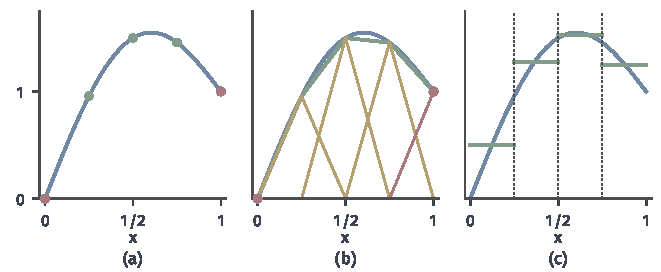
\includegraphics[width=112mm]{figures/06-differential-equations/02-partial-differential-equations/matplotlib/pdenum-three-unknowns/figure.pdf}
 \caption{同一个解$u=\sin(\pi x)+x$（蓝）的三种记录方式，$h=1/4$，红点是边值。(a)内部节点上的值（绿点）。(b)帽函数按节点值加权（黄线，右端红线是边界帽函数），其和是绿色折线。(c)四个单元上的平均（绿色水平线），虚线是单元界面。}
 \label{fig:pdenum-three-unknowns}
\end{BookInlineFigure}

把函数看成无限维向量，这三种做法都是在挑选有限个坐标：节点值是“按位置取样”，基函数系数是“在子空间里找坐标”，单元平均是“按小块累计”。类比到此为止，因为这三种坐标并不是同一个向量的不同分量，它们彼此之间相差一个与$h$有关的量。

例如在第一个单元$[0,1/4]$上，解的平均值由积分算出：
\[
 \bar{u}_1=4\int_0^{1/4}\bigl(\sin(\pi x)+x\bigr)\,\mathrm{d}x=\frac{4}{\pi}\Bigl(1-\frac{\sqrt2}{2}\Bigr)+\frac18\approx0.4979,
\]
而单元中点的值是$u(1/8)\approx0.5077$。比较数值解时必须说清比较的是哪一种量。

\paragraph{边界和初值怎样进入}
未知量选定后，还要说明已知数据放在哪里。Dirichlet边值是已知的节点值，它不再是未知量，而是把含它的项移到方程右端，右端因此带上边界数据。第~\ref{sec:pdenum-elliptic-fd}小节和第~\ref{sec:pdenum-weak-galerkin}小节会分别算出这一项。

Neumann条件和Robin条件规定的是边界通量。在弱形式和有限体积方法中，通量本来就在方程里出现，这些条件直接写进边界那一项；在差分格式中，则要用边界附近的差商或虚拟节点表达它们。

演化方程的初值$u_0$给出第一层数据，要按未知量的身份换算：差分取节点值，有限元取插值或投影，有限体积取单元平均。初值若不连续，这几种换算的差别并不小，后面的激波例子会用到单元平均。

\paragraph{三步离散，三份误差}
对演化方程，从$u$到屏幕上的数字要经过三步（图~\ref{fig:pdenum-error-pipeline}）。空间离散把场换成有限个未知量，得到第~\ref{chap:ode-numerical-methods}章讨论的常微分方程组；时间推进把它变成逐层的代数关系；每一层若含隐式方程，还要由有限精度的线性代数算出来。

\begin{BookInlineFigure}
 \centering
 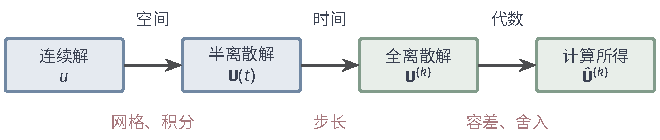
\includegraphics[width=112mm]{figures/06-differential-equations/02-partial-differential-equations/tikz/pdenum-error-pipeline/figure.pdf}
 \caption{从连续解到计算结果的三步。每个箭头引入一份误差，下方红字是控制它的主要因素。椭圆问题没有时间步，只有空间和代数两步。}
 \label{fig:pdenum-error-pipeline}
\end{BookInlineFigure}

记半离散解为$\bm{U}(t)$，全离散解为$\bm{U}^{(k)}$，实际算出的为$\widehat{\bm{U}}^{(k)}$，$\bm{R}_hu$表示把连续解按未知量的身份换算成离散向量。总误差分成三段：
\begin{equation}
 \begin{aligned}
 \bm{R}_hu(t_k)-\widehat{\bm{U}}^{(k)}
 &=\bigl(\bm{R}_hu(t_k)-\bm{U}(t_k)\bigr)\\
 &\quad+\bigl(\bm{U}(t_k)-\bm{U}^{(k)}\bigr)
 +\bigl(\bm{U}^{(k)}-\widehat{\bm{U}}^{(k)}\bigr).
 \end{aligned}
 \label{eq:pdenum-error-split}
\end{equation}

这样拆的好处是每一段可以单独控制，也可以单独检验。加密网格却不减小时间步，误差会停在时间误差的水平上；线性方程解得不够精确，误差会停在代数误差的水平上。第~\ref{sec:pdenum-error-cost}节会实际看到这两种停滞。

和常微分方程不同，这里步长变小时，向量$\bm{U}$的维数也在变。不同$h$对应的误差要能比较，范数必须随网格换算，比如$\lVert\bm{v}\rVert_{2,h}=(h\sum_jv_j^2)^{1/2}$相当于$L^2$范数，而$\lVert\bm{v}\rVert_\infty$相当于最大模。不带因子$h$的欧氏范数会随未知量增多而变大，不能用来比较。

\section{有限差分}
\label{sec:pdenum-finite-differences}

导数是极限，极限是算不完的，能算的是相邻几个值的差商。差商和导数差多少，由Taylor展开回答。

设$u$在$x$附近足够光滑。把$u(x\pm h)$在$x$处展开：
\[
 u(x\pm h)=u(x)\pm hu'(x)+\frac{h^2}{2}u''(x)\pm\frac{h^3}{6}u'''(x)+\frac{h^4}{24}u''''(\xi_\pm).
\]

只用一侧的值，得到前向差商和后向差商，它们与$u'(x)$相差$O(h)$。两式相减，偶次项消去，得到中心差商：
\begin{equation}
 \frac{u(x+h)-u(x-h)}{2h}=u'(x)+O(h^2).
 \label{eq:pdenum-central-first}
\end{equation}

两式相加，奇次项消去，得到二阶导数的三点公式：
\begin{equation}
 \delta_h^2u(x):=\frac{u(x-h)-2u(x)+u(x+h)}{h^2}=u''(x)+\frac{h^2}{12}u''''(\xi),
 \label{eq:pdenum-second-difference}
\end{equation}
其中$\xi\in(x-h,x+h)$，这里用到$u\in C^4$和介值定理，把两个余项合并成一个。

图~\ref{fig:pdenum-taylor-stencil}用$u=x^3$在$x=1$、$h=1/2$处比较三条割线。切线斜率是$3$，前向差商是$4.75$，后向差商是$1.75$，中心差商是$3.25$。两侧的偏差方向相反，取平均时一阶项抵消。

\begin{BookInlineFigure}
 \centering
 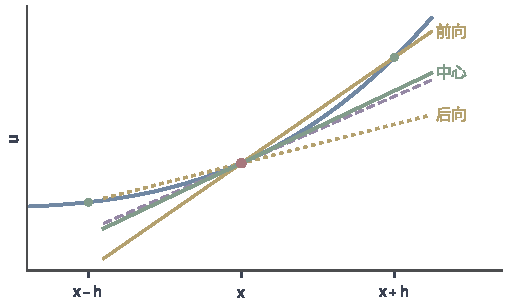
\includegraphics[width=86mm]{figures/06-differential-equations/02-partial-differential-equations/matplotlib/pdenum-taylor-stencil/figure.pdf}
 \caption{$u=x^3$（蓝）在红点$x=1$处的切线（紫色虚线）与三条差商割线，$h=1/2$。前向和后向差商（黄）分别偏大和偏小，中心差商（绿）的斜率$3.25$最接近切线的斜率$3$。}
 \label{fig:pdenum-taylor-stencil}
\end{BookInlineFigure}

余项里的$u''''$提醒我们：“二阶精度”不是公式本身的性质，而是公式加上解的光滑性的结论。解不够光滑时，式~\eqref{eq:pdenum-second-difference}的余项估计不成立，下面会看到实际阶数随之下降。

\subsection{椭圆方程的差分}
\label{sec:pdenum-elliptic-fd}

\paragraph{主要思想}
方程~\eqref{eq:pdenum-model}要求在每个内部节点$x_j$处成立，现在把它换成相邻三个节点值之间的关系。由式~\eqref{eq:pdenum-second-difference}，在$j=1,\ldots,n-1$上要求
\begin{equation}
 \frac{-U_{j-1}+2U_j-U_{j+1}}{h^2}=f(x_j),\qquad U_0=g_0,\quad U_n=g_1 .
 \label{eq:pdenum-three-point}
\end{equation}
这是$n-1$个未知量的线性方程组$\bm{A}_h\bm{U}=\bm{b}$。

边值出现在第一个和最后一个方程里。$j=1$的方程含已知的$U_0$，$j=n-1$的方程含已知的$U_n$，把它们移到右端，得到
\begin{equation}
 \bm{A}_h=\frac{1}{h^2}\begin{bmatrix}2&-1&&\\-1&2&\ddots&\\&\ddots&\ddots&-1\\&&-1&2\end{bmatrix},\qquad
 \bm{b}=\begin{bmatrix}f(x_1)+g_0/h^2\\f(x_2)\\\vdots\\f(x_{n-1})+g_1/h^2\end{bmatrix}.
 \label{eq:pdenum-fd-system}
\end{equation}

$\bm{A}_h$是三对角矩阵，按未知量的顺序消元时不产生新的非零元。一般的分解算法可参考\BookChapterRef{chap:direct-linear-solvers}{卷二第12章“线性方程的直接求解”}，这里只需要它的三对角形式。记对角元为$a_j$，上、下次对角元为$e_j$和$l_j$。消去第$j$行的下次对角元，逐行得到
\begin{equation}
 m_j=\frac{l_j}{d_{j-1}},\qquad d_j=a_j-m_je_{j-1},\qquad y_j=b_j-m_jy_{j-1}.
 \label{eq:pdenum-thomas-forward}
\end{equation}
消元后方程变成上双对角，再从最后一行往回代入：
\begin{equation}
 U_{n-1}=\frac{y_{n-1}}{d_{n-1}},\qquad U_j=\frac{y_j-e_jU_{j+1}}{d_j}.
 \label{eq:pdenum-thomas-back}
\end{equation}

\needspace{6\baselineskip}
\paragraph{变量}
\begin{itemize}
 \item $h=1/n$：步长；$x_j=jh$：节点，$j=0,\ldots,n$。
 \item $\bm{A}_h$：$(n-1)\times(n-1)$三对角矩阵，存为三个长度约$n$的数组。
 \item $\bm{b}\in\mathbb{R}^{n-1}$：节点上的右端，已含边值贡献。
 \item $d_j,y_j$：消元过程中的对角元和右端；$\bm{U}\in\mathbb{R}^{n-1}$：节点上的近似解。
\end{itemize}

\paragraph{初始化}
按式~\eqref{eq:pdenum-fd-system}填入$\bm{A}_h$与$\bm{b}$，并令$d_1=a_1$，$y_1=b_1$。

例中取$n=4$，$h=1/4$，$1/h^2=16$，$g_0=0$，$g_1=1$。节点上$f(x_j)=\pi^2\sin(\pi x_j)$，第三个方程的右端再加上$g_1/h^2=16$，于是
\[
 \bm{A}_h=16\begin{bmatrix}2&-1&0\\-1&2&-1\\0&-1&2\end{bmatrix},\qquad
 \bm{b}=\begin{bmatrix}6.9789\\9.8696\\22.9789\end{bmatrix}.
\]
初值是$d_1=32$，$y_1=6.9789$。

\needspace{6\baselineskip}
\paragraph{每轮更新}
对$j=2,\ldots,n-1$依次执行下面两步，第$n-1$行处理完后结束消元。
\begin{enumerate}
 \item 由式~\eqref{eq:pdenum-thomas-forward}算出$m_j,d_j$。例中第一轮$j=2$，第二轮$j=3$：
 \[
  \begin{aligned}
  m_2&=\frac{-16}{32}=-0.5, & d_2&=32-(-0.5)(-16)=24,\\
  m_3&=\frac{-16}{24}=-0.6667, & d_3&=32-(-0.6667)(-16)=21.3333.
  \end{aligned}
 \]
 \item 由同一式更新右端。例中两轮分别是
 \[
  \begin{aligned}
  y_2&=9.8696+0.5\times6.9789=13.3590,\\
  y_3&=22.9789+0.6667\times13.3590=31.8849.
  \end{aligned}
 \]
\end{enumerate}

消元结束后按式~\eqref{eq:pdenum-thomas-back}从下往上回代。例中依次得到
\[
 U_3=\frac{31.8849}{21.3333}=1.4946,\qquad
 U_2=\frac{13.3590+16\times1.4946}{24}=1.5530,
\]
\[
 U_1=\frac{6.9789+16\times1.5530}{32}=0.9946.
\]

最终得到节点上的近似解$(0.9946,\,1.5530,\,1.4946)$。式~\eqref{eq:pdenum-model-exact}给出的真值是$(0.9571,\,1.5000,\,1.4571)$，三个误差依次为$0.0375$、$0.0530$、$0.0375$。

\begin{BookInlineFigure}
 \centering
 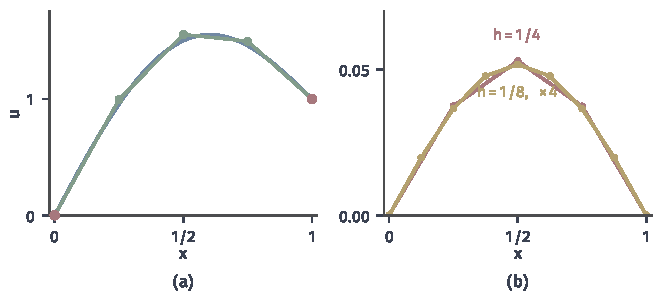
\includegraphics[width=112mm]{figures/06-differential-equations/02-partial-differential-equations/matplotlib/pdenum-fd-solution/figure.pdf}
 \caption{三点格式解问题~\eqref{eq:pdenum-model}。(a)$h=1/4$的数值解（绿）与真解（蓝），红点是边值。(b)节点误差，红线为$h=1/4$，黄线为$h=1/8$的误差乘以$4$：两条折线几乎重合，说明误差按$h^2$减小。}
 \label{fig:pdenum-fd-solution}
\end{BookInlineFigure}

图~\ref{fig:pdenum-fd-solution}(b)显示步长减半时误差约变为四分之一。这件事为什么成立？每个方程的残差很小，并不直接说明解的误差很小，下面要把两者联系起来。

\paragraph{从残差到误差}
把真解的节点值$\bm{R}_hu$代入离散方程，方程不再精确成立，差值就是\term{截断误差}（truncation error）：
\begin{equation}
 \bm{\tau}_h=\bm{A}_h\bm{R}_hu-\bm{b}.
 \label{eq:pdenum-truncation}
\end{equation}
由式~\eqref{eq:pdenum-second-difference}，$u\in C^4[0,1]$时它的每个分量满足$\lvert\tau_j\rvert\leq h^2M_4/12$，其中$M_4=\max\lvert u''''\rvert$。

离散解的误差$\bm{e}=\bm{R}_hu-\bm{U}$满足$\bm{A}_h\bm{e}=\bm{\tau}_h$，所以$\bm{e}=\bm{A}_h^{-1}\bm{\tau}_h$。问题归结为$\bm{A}_h^{-1}$的大小，而且这个大小不能随$h$变小而变大。这里要注意，$\bm{A}_h$的元素是$h^{-2}$量级，直接看它的元素说明不了逆的大小。

连续问题中，最大值原理控制了$-u''=f$的解（第~\ref{chap:elliptic-equations}章）。离散问题有完全平行的结论，证明也更短，因为“最大值点”只需在有限个数里找。

\begin{theorem}[离散最大值原理]
 \label{thm:pdenum-discrete-maximum}
 设网格函数$v_0,\ldots,v_n$在每个内部节点满足
 \begin{equation}
  \frac{-v_{j-1}+2v_j-v_{j+1}}{h^2}\leq0,\qquad j=1,\ldots,n-1,
  \label{eq:pdenum-discrete-subharmonic}
 \end{equation}
 则$\max_jv_j=\max(v_0,v_n)$。
\end{theorem}

\begin{proof}
 设最大值$M$在某个内部节点$j$取到。条件~\eqref{eq:pdenum-discrete-subharmonic}可以写成
 \[
  v_j\leq\frac{v_{j-1}+v_{j+1}}{2}.
 \]
 两个邻点都不超过$M$，而它们的平均不小于$v_j=M$，所以两个邻点都等于$M$。

 对邻点重复这个论证，最大值一路传到端点，于是$v_0=M$（也有$v_n=M$）。若最大值不在内部取到，它已经在端点上。
\end{proof}

这个定理的直观内容与热的抹平一致：每一点都不高于两邻点的平均，就不可能自己鼓起一个包。用它可以估计逆矩阵，诀窍是找一个差分算子作用后恰好等于$1$的函数。

\begin{theorem}[三点格式的误差界]
 \label{thm:pdenum-fd-error}
 对任意$\bm{\tau}\in\mathbb{R}^{n-1}$，$\bm{A}_h\bm{e}=\bm{\tau}$的解满足
 \begin{equation}
  \lVert\bm{e}\rVert_\infty\leq\frac18\lVert\bm{\tau}\rVert_\infty .
  \label{eq:pdenum-inverse-bound}
 \end{equation}
 若问题的解$u\in C^4[0,1]$，则
 \begin{equation}
  \max_j\lvert u(x_j)-U_j\rvert\leq\frac{h^2}{96}\max_{[0,1]}\lvert u''''\rvert .
  \label{eq:pdenum-fd-error}
 \end{equation}
\end{theorem}

\begin{proof}
 取$w(x)=x(1-x)/2$。它是二次函数，式~\eqref{eq:pdenum-second-difference}的余项为零，所以$-\delta_h^2w=-w''=1$，即$w$的节点值满足$\bm{A}_hw=\bm{1}$。

 令$v_j=e_j-\lVert\bm{\tau}\rVert_\infty w(x_j)$，并约定$e_0=e_n=0$。则$v_0=v_n=0$，且在内部节点上
 \[
  \frac{-v_{j-1}+2v_j-v_{j+1}}{h^2}=\tau_j-\lVert\bm{\tau}\rVert_\infty\leq0 .
 \]

 由定理~\ref{thm:pdenum-discrete-maximum}，$v_j\leq0$，即$e_j\leq\lVert\bm{\tau}\rVert_\infty w(x_j)$。对$-\bm{e}$作同样的论证，得到
 \[
  \lvert e_j\rvert\leq\lVert\bm{\tau}\rVert_\infty w(x_j) .
 \]

 $w$的最大值是$w(1/2)=1/8$，式~\eqref{eq:pdenum-inverse-bound}成立。把$\lVert\bm{\tau}_h\rVert_\infty\leq h^2M_4/12$代入，得到式~\eqref{eq:pdenum-fd-error}。
\end{proof}

证明的结构是后面反复出现的模式：一致性给出小的残差，稳定性（这里是$\lVert\bm{A}_h^{-1}\rVert_\infty\leq1/8$，常数与$h$无关）把残差转成解的误差。

例中$u''''=\pi^4\sin(\pi x)$，$M_4=\pi^4$，表~\ref{tab:pdenum-fd-refine}比较实际误差与上界。

\begin{BookInlineTable}
 \centering
 \caption{三点格式解问题~\eqref{eq:pdenum-model}的最大模误差和式~\eqref{eq:pdenum-fd-error}的上界。}
 \label{tab:pdenum-fd-refine}
 \begin{tabular}{cccc}
  \toprule
  $n$ & 实际误差 & 上界 & 相邻误差之比\\
  \midrule
  $4$ & $5.303\times10^{-2}$ & $6.342\times10^{-2}$ & --\\
  $8$ & $1.295\times10^{-2}$ & $1.585\times10^{-2}$ & $4.09$\\
  $16$ & $3.219\times10^{-3}$ & $3.964\times10^{-3}$ & $4.02$\\
  $32$ & $8.036\times10^{-4}$ & $9.909\times10^{-4}$ & $4.01$\\
  \bottomrule
 \end{tabular}
\end{BookInlineTable}

\paragraph{光滑性不够时}
误差界要求$u\in C^4$。换一个解$u=x^{3/2}-x$，它满足$u(0)=u(1)=0$，源项$f=-\tfrac34x^{-1/2}$在内部节点上有定义，但$u''$在$x=0$处无界，定理的条件不满足。

\begin{BookInlineFigure}
 \centering
 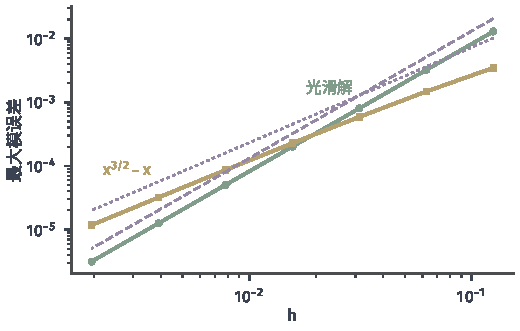
\includegraphics[width=88mm]{figures/06-differential-equations/02-partial-differential-equations/matplotlib/pdenum-fd-rates/figure.pdf}
 \caption{三点格式的网格加密，$n$从$8$到$512$，绿线是光滑解$\sin(\pi x)+x$，黄线是$x^{3/2}-x$。紫色虚线是斜率$2$，紫色点线是斜率$3/2$的参考线。公式没有改变，实际的收敛阶却取决于解的光滑性。}
 \label{fig:pdenum-fd-rates}
\end{BookInlineFigure}

图~\ref{fig:pdenum-fd-rates}是实际结果。光滑解每次加密的观测阶稳定在$2.00$附近。$x^{3/2}-x$的观测阶依次为$1.23$、$1.33$、$1.37$、$1.40$、$1.43$、$1.44$，逐渐向$3/2$靠近。这就是不能只凭公式形式判断精度的原因。

\paragraph{规则网格上的Poisson格式}
到两个空间维，在单位正方形上取步长$h$的规则网格。把$x_1$方向和$x_2$方向的三点公式相加，得到五点公式：
\begin{equation}
 \frac{4U_{i,j}-U_{i-1,j}-U_{i+1,j}-U_{i,j-1}-U_{i,j+1}}{h^2}=f(\bm{x}_{i,j}) .
 \label{eq:pdenum-five-point}
\end{equation}

边界上的节点值已知，出现时同样移到右端。图~\ref{fig:pdenum-five-point}(a)是模板的系数，(b)是$h=1/3$的网格，只有绿色的四个节点是未知量。

\begin{BookInlineFigure}
 \centering
 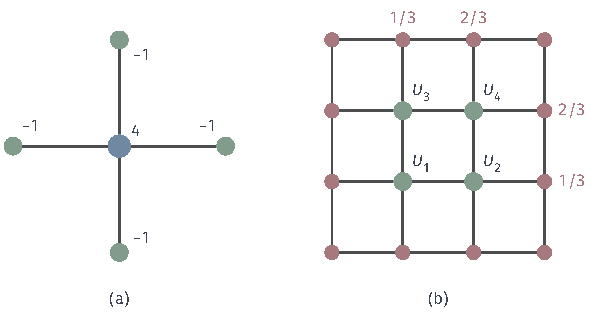
\includegraphics[width=101mm]{figures/06-differential-equations/02-partial-differential-equations/tikz/pdenum-five-point/figure.pdf}
 \caption{(a)五点模板，中心系数$4$，四个邻点系数$-1$，整体除以$h^2$。(b)$h=1/3$的网格，绿点是未知量，红点是已知的边值。边界标注是例子中边值$g=x_1x_2$在右边和上边的取值，左边和下边$g=0$。}
 \label{fig:pdenum-five-point}
\end{BookInlineFigure}

取$-\Delta u=0$，边值$g=x_1x_2$，真解就是$u=x_1x_2$。按图中编号，例如$U_2$的方程含右邻的边值$g(1,1/3)=1/3$，$U_4$的方程含右邻$g(1,2/3)$和上邻$g(2/3,1)$。乘以$h^2$并把边值移到右端，方程组是
\begin{equation}
 \begin{bmatrix}4&-1&-1&0\\-1&4&0&-1\\-1&0&4&-1\\0&-1&-1&4\end{bmatrix}
 \begin{bmatrix}U_1\\U_2\\U_3\\U_4\end{bmatrix}
 =\begin{bmatrix}0\\1/3\\1/3\\4/3\end{bmatrix}.
 \label{eq:pdenum-five-point-example}
\end{equation}

利用对称性$U_2=U_3$。第一个方程给出
\[
 U_2=2U_1 .
\]
代入第二个方程，得到
\[
 U_4=7U_1-\frac13 .
\]
最后一个方程成为$4U_4-2U_2=4/3$，代入上面两式，
\[
 24U_1=\frac83,\qquad U_1=\frac19,\quad U_2=U_3=\frac29,\quad U_4=\frac49 .
\]
这正是$x_1x_2$在四个节点上的值。原因是$x_1x_2$的四阶导数全为零，截断误差为零。

一般情形的误差估计与一维相同。设$u\in C^4(\overline{\Omega})$，比较函数仍取$w=x_1(1-x_1)/2$，它在五点算子下也给出$1$，所以$\lVert\bm{A}_h^{-1}\rVert_\infty\leq1/8$，最大模误差不超过$(h^2/96)(\max\lvert\partial_1^4u\rvert+\max\lvert\partial_2^4u\rvert)$。

矩阵的结构发生了变化。图~\ref{fig:pdenum-matrix-pattern}中，一维矩阵的非零元贴着对角线，二维矩阵除三条对角线外，还有两条离对角线一整行网格之远的带。按行消元时，带内的零元会被填满，所以二维问题的直接分解远比一维昂贵，第~\ref{sec:pdenum-error-cost}节再讨论这个代价。

\begin{BookInlineFigure}
 \centering
 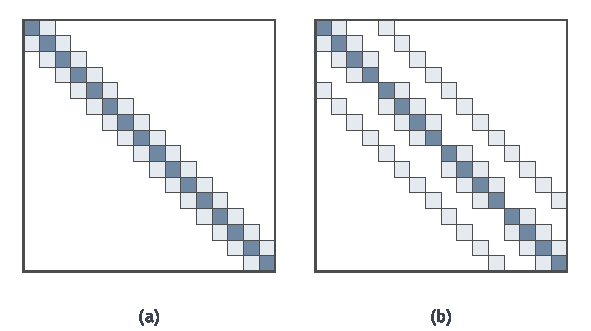
\includegraphics[width=100mm]{figures/06-differential-equations/02-partial-differential-equations/matplotlib/pdenum-matrix-pattern/figure.pdf}
 \caption{差分矩阵的非零元位置，深色是对角元。(a)一维三点格式，$16$个未知量。(b)二维五点格式，$4\times4$个内部节点，共$16$个未知量，按行编号。这里的方格本身是矩阵元素。}
 \label{fig:pdenum-matrix-pattern}
\end{BookInlineFigure}

规则网格的方便之处也是限制。边界不沿网格线时，靠近边界的节点需要专门的不等距模板，矩阵的对称性和最大值性质都要重新检查。下一节的有限元方法从弱形式出发，处理一般区域要自然得多。

\subsection{扩散方程的差分}
\label{sec:pdenum-heat-fd}

现在让温度随时间变化。考虑
\begin{equation}
 \partial_tu=\partial_x^2u\quad\text{于}\ (0,1)\times(0,T],\qquad u(0,t)=u(1,t)=0,\quad u(x,0)=u_0(x).
 \label{eq:pdenum-heat}
\end{equation}
这里只对空间做上一小节的离散，把时间留到下一步，这种做法称为\term{半离散}（semi-discretization）。

\paragraph{主要思想}
在内部节点上用三点公式代替$\partial_x^2u$，时间仍然连续，就得到常微分方程组
\begin{equation}
 \dot{\bm{U}}(t)=-\bm{A}_h\bm{U}(t),\qquad \bm{U}(0)=\bm{R}_hu_0 .
 \label{eq:pdenum-semidiscrete}
\end{equation}
偏微分方程变成了第~\ref{chap:ode-numerical-methods}章的线性系统，这正是把函数看成无限维向量所期待的对应：算子$\partial_x^2$对应矩阵$-\bm{A}_h$，它的特征模式对应矩阵的特征向量。

矩阵的特征向量恰好是正弦函数在节点上的取样。用三角恒等式
\[
 \sin(m\pi(j-1)h)+\sin(m\pi(j+1)h)=2\cos(m\pi h)\sin(m\pi jh)
\]
代入，得到$\bm{A}_h$的特征值
\begin{equation}
 \lambda_m=\frac{4}{h^2}\sin^2\frac{m\pi h}{2},\qquad m=1,\ldots,n-1 .
 \label{eq:pdenum-discrete-eigenvalues}
\end{equation}

$h\to0$时对固定的$m$有$\lambda_m\to m^2\pi^2$，这是连续算子的特征值。但$m$接近$n$时情形完全不同：最大特征值$\lambda_{n-1}=(4/h^2)\cos^2(\pi h/2)$接近$4/h^2$。

\begin{BookInlineFigure}
 \centering
 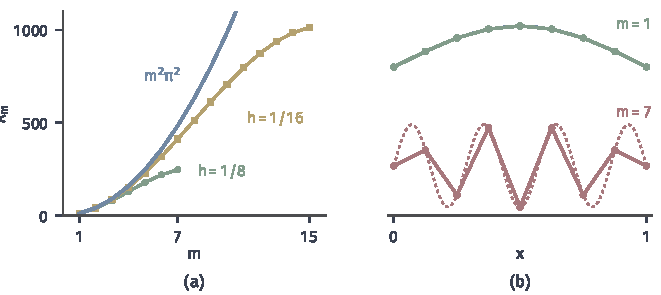
\includegraphics[width=112mm]{figures/06-differential-equations/02-partial-differential-equations/matplotlib/pdenum-heat-modes/figure.pdf}
 \caption{(a)连续特征值$m^2\pi^2$（蓝）与差分矩阵的特征值（绿$h=1/8$，黄$h=1/16$）。低模式贴近蓝线，高模式明显偏低，而网格越细，最大特征值越大。(b)$h=1/8$上的两个模式，绿线$m=1$，红线$m=7$；虚线是对应的连续正弦。}
 \label{fig:pdenum-heat-modes}
\end{BookInlineFigure}

图~\ref{fig:pdenum-heat-modes}说明了网格变细时发生的事。网格加密引入了越来越快的衰减模式，这些锯齿模式在真解中早已消失，也不是我们想算的东西，却决定了显式方法的步长上限。这与第~\ref{chap:ode-numerical-methods}章的刚性问题是同一件事。

在时间方向上，用步长$\tau$对式~\eqref{eq:pdenum-semidiscrete}作三种推进。三者的迭代公式为
\begin{align}
 \bm{U}^{(k+1)}&=(\bm{I}-\tau\bm{A}_h)\bm{U}^{(k)},
 \label{eq:pdenum-ftcs}\\
 \bm{U}^{(k+1)}&=(\bm{I}+\tau\bm{A}_h)^{-1}\bm{U}^{(k)},
 \label{eq:pdenum-btcs}\\
 \bm{U}^{(k+1)}&=\Bigl(\bm{I}+\frac{\tau}{2}\bm{A}_h\Bigr)^{-1}\Bigl(\bm{I}-\frac{\tau}{2}\bm{A}_h\Bigr)\bm{U}^{(k)}.
 \label{eq:pdenum-cn}
\end{align}
它们依次是显式Euler方法、后向Euler方法和\term{Crank--Nicolson方法}（Crank--Nicolson method）。第三种是梯形方法用在式~\eqref{eq:pdenum-semidiscrete}上的结果。

记$r=\tau/h^2$，式~\eqref{eq:pdenum-ftcs}的分量形式是
\begin{equation}
 U_j^{(k+1)}=U_j^{(k)}+r\bigl(U_{j-1}^{(k)}-2U_j^{(k)}+U_{j+1}^{(k)}\bigr).
 \label{eq:pdenum-ftcs-component}
\end{equation}

\needspace{6\baselineskip}
\paragraph{变量}
\begin{itemize}
 \item $\bm{U}^{(k)}\in\mathbb{R}^{n-1}$：第$k$层内部节点上的近似值。
 \item $h,\tau,r=\tau/h^2$：空间步、时间步及它们的比值。
 \item 后向Euler方法和Crank--Nicolson方法还要保存三对角矩阵及其消元结果$d_j$。
\end{itemize}

\paragraph{初始化}
令$U_j^{(0)}=u_0(x_j)$。例中取$h=1/4$，$u_0=\sin(\pi x)+0.1\sin(3\pi x)$，由它的两个模式可以写出真解：
\begin{equation}
 u(x,t)=\mathrm{e}^{-\pi^2t}\sin(\pi x)+0.1\,\mathrm{e}^{-9\pi^2t}\sin(3\pi x).
 \label{eq:pdenum-heat-exact}
\end{equation}
三个节点上的初值是
\[
 \bm{U}^{(0)}=(0.7778,\,0.9000,\,0.7778)^\top .
\]

\needspace{6\baselineskip}
\paragraph{每轮更新}
显式格式每轮按式~\eqref{eq:pdenum-ftcs-component}对$j=1,\ldots,n-1$算一遍，边界值$U_0=U_n=0$不更新，到$k\tau=T$结束。

例中先取$\tau=0.03$，$r=0.48$。第一轮中间节点的值是
\[
 U_2^{(1)}=0.9+0.48(0.7778-1.8+0.7778)=0.7827,
\]
左节点的值是
\[
 U_1^{(1)}=0.7778+0.48(0-1.5556+0.9)=0.4631 .
\]
此后各轮的结果为
\[
 \begin{aligned}
 \bm{U}^{(1)}&=(0.4631,\,0.7827,\,0.4631)^\top,\\
 \bm{U}^{(2)}&=(0.3942,\,0.4759,\,0.3942)^\top,\\
 \bm{U}^{(3)}&=(0.2442,\,0.3975,\,0.2442)^\top.
 \end{aligned}
\]
数值解有些摆动，但在衰减。把时间步改成$\tau=0.05$，$r=0.8$，前四轮是
\[
 \begin{aligned}
 \bm{U}^{(1)}&=(0.2533,\,0.7045,\,0.2533)^\top,\\
 \bm{U}^{(2)}&=(0.4116,\,-0.0174,\,0.4116)^\top,\\
 \bm{U}^{(3)}&=(-0.2609,\,0.6690,\,-0.2609)^\top,\\
 \bm{U}^{(4)}&=(0.6918,\,-0.8189,\,0.6918)^\top.
 \end{aligned}
\]
真解在$t=0.2$时中点的值是$0.1389$，而数值解已经变号并开始放大。

后向Euler方法每轮解一个三对角方程，用式~\eqref{eq:pdenum-thomas-forward}和式~\eqref{eq:pdenum-thomas-back}，矩阵的对角元是$1+2r$，次对角元是$-r$。例中$\tau=0.05$，$r=0.8$，第一轮的消元过程是
\[
 \begin{aligned}
 m_2&=-0.3077, & d_2&=2.3538, & y_2&=1.1393,\\
 m_3&=-0.3399, & d_3&=2.3281, & y_3&=1.1650,
 \end{aligned}
\]
从$d_1=2.6$和$y_1=0.7778$出发。回代给出
\[
 \bm{U}^{(1)}=(0.5004,\,0.6541,\,0.5004)^\top .
\]
第二、第三轮分别得到中点值$0.4565$和$0.3138$。同一个$\tau$下，Crank--Nicolson方法前三轮的中点值是$0.6358$、$0.3824$、$0.2391$，而真解是$0.6093$、$0.3727$、$0.2275$。它们都不放大。最终得到的是一列随时间衰减的向量，比较结果见下面对放大因子的分析。

\paragraph{放大因子解释一切}
对每个模式，$-\tau\lambda_m=z$，三种格式分别把这个模式乘上
\begin{equation}
 R_{\mathrm{E}}(z)=1+z,\qquad R_{\mathrm{B}}(z)=\frac{1}{1-z},\qquad R_{\mathrm{CN}}(z)=\frac{1+z/2}{1-z/2}.
 \label{eq:pdenum-heat-factors}
\end{equation}

例中$\lambda_1,\lambda_2,\lambda_3$分别约为$9.37$、$32$、$54.63$。$\tau=0.05$时，$R_{\mathrm{E}}$在三个模式上取$0.531$、$-0.6$、$-1.731$，第三个模式的绝对值大于$1$，放大的正是这个模式；$\tau=0.03$时，三个值是$0.719$、$0.04$、$-0.639$。图~\ref{fig:pdenum-amplification}把三条放大因子曲线和例中的点画在一起。

\begin{BookInlineFigure}
 \centering
 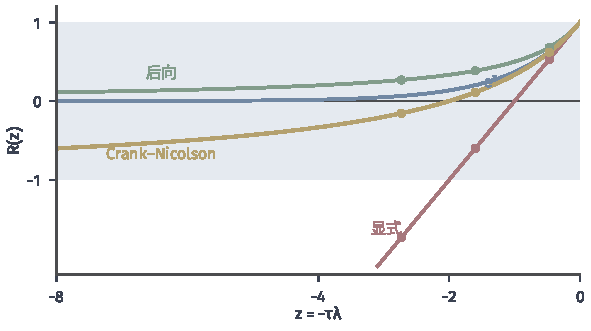
\includegraphics[width=100mm]{figures/06-differential-equations/02-partial-differential-equations/matplotlib/pdenum-amplification/figure.pdf}
 \caption{负实轴上的放大因子：蓝线是真解的$\mathrm{e}^{z}$，红线是显式Euler方法，绿线是后向Euler方法，黄线是Crank--Nicolson方法。浅蓝带表示$\lvert R\rvert\leq1$。圆点是$h=1/4$，$\tau=0.05$时三个模式的$z$值，显式Euler方法最左边的红点已在带外。}
 \label{fig:pdenum-amplification}
\end{BookInlineFigure}

显式格式要求所有模式都有$\lvert1+z\rvert\leq1$，即
\begin{equation}
 \tau\lambda_{\max}\leq2 .
 \label{eq:pdenum-ftcs-stability}
\end{equation}
由于$\lambda_{\max}<4/h^2$，$r=\tau/h^2\leq1/2$对任何网格都足够。例中$2/\lambda_{\max}=0.0366$，所以$\tau=0.03$稳定，$\tau=0.05$不稳定。

图~\ref{fig:pdenum-heat-stability}在$h=1/20$上比较阈值两侧。初值加了一个$2\times10^{-5}$大小的锯齿模式，它代表实际计算中总会出现的微小扰动。$r=0.55$时，这个几乎看不见的模式每步放大约$1.19$倍，到$t=0.08$时已经把解淹没。

\begin{BookInlineFigure}
 \centering
 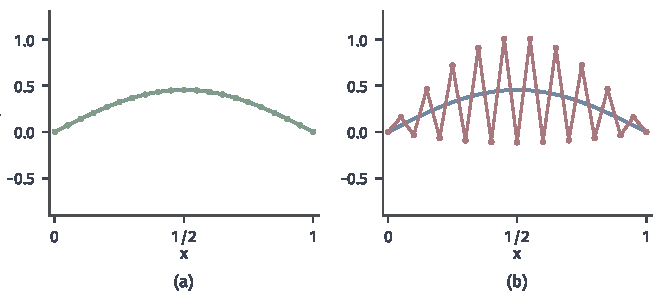
\includegraphics[width=112mm]{figures/06-differential-equations/02-partial-differential-equations/matplotlib/pdenum-heat-stability/figure.pdf}
 \caption{显式Euler方法在$h=1/20$上解式~\eqref{eq:pdenum-heat}到$t=0.08$，蓝线是真解。初值$\sin(\pi x)+0.1\sin(3\pi x)$叠加了幅度$2\times10^{-5}$的$\sin(19\pi x)$。(a)$r=0.4$，绿线贴合真解。(b)$r=0.55$，红线成为节点间振荡的锯齿。}
 \label{fig:pdenum-heat-stability}
\end{BookInlineFigure}

后向Euler方法对任何$z<0$都有$0<R_{\mathrm{B}}<1$，Crank--Nicolson方法也有$\lvert R_{\mathrm{CN}}\rvert<1$，它们都是无条件稳定的。但两者并不等价。$z\to-\infty$时，$R_{\mathrm{B}}\to0$，$R_{\mathrm{CN}}\to-1$，也就是说Crank--Nicolson方法几乎不衰减高模式，只是让它们每步变号。

\begin{BookInlineFigure}
 \centering
 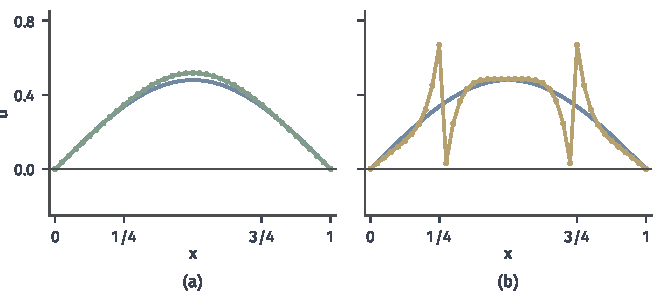
\includegraphics[width=112mm]{figures/06-differential-equations/02-partial-differential-equations/matplotlib/pdenum-cn-oscillation/figure.pdf}
 \caption{方波初值、$h=1/40$、$\tau=0.02$（$r=32$）走三步。蓝线是半离散系统的精确解。(a)后向Euler方法（绿）光滑，略有偏差。(b)Crank--Nicolson方法（黄）在间断附近保留了振荡，此时最高模式的放大因子约为$-0.97$。}
 \label{fig:pdenum-cn-oscillation}
\end{BookInlineFigure}

图~\ref{fig:pdenum-cn-oscillation}是这个差别的后果。初值的跳跃含有大量高模式，$r$很大时，Crank--Nicolson方法在跳跃处留下不衰减的尖峰，而真解在第一瞬间就把它们抹平了。“无条件稳定”只是说不放大，并不保证解的外观正确。

\paragraph{精度和稳定对步长的不同要求}
稳定性问的是误差会不会放大，精度问的是每步新引入多少误差。Taylor展开给出三种格式的截断误差：两种Euler方法是$O(\tau+h^2)$，Crank--Nicolson方法是$O(\tau^2+h^2)$。要让时间误差和空间误差平衡，所需的步长并不一样，表~\ref{tab:pdenum-heat-steps}汇总了这一点和实际的误差。

\begin{BookInlineTable}
 \centering
 \caption{热方程$u_0=\sin(\pi x)$到$T=0.1$的最大模误差。表头括号内是时间步的选取。}
 \label{tab:pdenum-heat-steps}
 \begin{tabular}{ccccc}
  \toprule
  $n$ & 显式（$r=0.4$） & 后向（$\tau=h$） & 后向（$\tau=h^2$） & CN（$\tau=h$）\\
  \midrule
  $10$ & $4.29\times10^{-3}$ & $1.33\times10^{-1}$ & $2.03\times10^{-2}$ & $2.99\times10^{-2}$\\
  $20$ & $1.06\times10^{-3}$ & $7.62\times10^{-2}$ & $5.24\times10^{-3}$ & $6.88\times10^{-3}$\\
  $40$ & $2.65\times10^{-4}$ & $4.14\times10^{-2}$ & $1.32\times10^{-3}$ & $1.69\times10^{-3}$\\
  $80$ & $6.62\times10^{-5}$ & $2.16\times10^{-2}$ & $3.31\times10^{-4}$ & $4.20\times10^{-4}$\\
  \bottomrule
 \end{tabular}
\end{BookInlineTable}

显式格式的$\tau\sim h^2$是稳定性强加的，时间精度因此多余。后向Euler方法稳定性上没有限制，但要达到$O(h^2)$，精度仍然要求$\tau\sim h^2$，表中$\tau=h$一列只有一阶收敛。Crank--Nicolson方法取$\tau\sim h$就够了，代价是对粗糙数据要小心。

二维和三维的规则网格上，$\lambda_{\max}$约为$4d/h^2$，显式稳定条件变成$r\leq1/(2d)$。同样地，这些稳定性结论都依赖矩阵的对称结构和这里的边界处理，第~\ref{sec:pdenum-stability}节回到这个问题。

\section{Galerkin有限元}
\label{sec:pdenum-galerkin}

差分方法直接逼近导数，要求解有足够多的导数，网格也最好是规则的。第~\ref{chap:elliptic-equations}章的弱形式提供了另一个出发点：方程只需对一族测试函数成立，一阶导数就够了。于是可以换一个问法，不再逼近导数，而是在一个有限维的函数空间里找最好的近似。

这里只讨论二阶椭圆问题。一般泛函的Ritz思想可参考\BookChapterRef{chap:functional-optimization-variation}{卷五第29章“泛函优化”}，本节着重处理边界条件、局部基函数和方程误差。

\subsection{离散弱问题}
\label{sec:pdenum-weak-galerkin}

\paragraph{把试探空间换成有限维}
回忆第~\ref{chap:elliptic-equations}章的抽象形式。设$V$是Hilbert空间，对齐次Dirichlet问题是$H^1_0(\Omega)$；$a$是$V$上的双线性型，$\ell$是$V$上的有界线性泛函。弱问题是求$u\in V$，使
\begin{equation}
 a(u,v)=\ell(v)\qquad\text{对所有}\ v\in V .
 \label{eq:pdenum-weak}
\end{equation}
对问题$-\Delta u=f$，两个对象分别是
\[
 a(u,v)=\int_\Omega\nabla u\cdot\nabla v\,\mathrm{d}\bm{x},\qquad \ell(v)=\int_\Omega fv\,\mathrm{d}\bm{x}.
\]

式~\eqref{eq:pdenum-weak}要对无穷多个$v$成立，未知量$u$也在无穷维空间里。Galerkin的办法是同时限制两者：取有限维子空间$V_h\subset V$，把试探函数和测试函数都取在$V_h$中。

\begin{definition}[Galerkin方程]
 \label{def:pdenum-galerkin}
 设$V_h\subset V$是有限维子空间。求$u_h\in V_h$，使
 \begin{equation}
  a(u_h,v_h)=\ell(v_h)\qquad\text{对所有}\ v_h\in V_h .
  \label{eq:pdenum-galerkin}
 \end{equation}
 $V_h\subset V$这个包含关系称为\term{协调性}（conformity）。
\end{definition}

取$V_h$的基$\varphi_1,\ldots,\varphi_N$，写$u_h=\sum_jc_j\varphi_j$，并依次取$v_h=\varphi_i$。由双线性，式~\eqref{eq:pdenum-galerkin}等价于线性方程组
\begin{equation}
 \bm{K}\bm{c}=\bm{b},\qquad K_{ij}=a(\varphi_j,\varphi_i),\quad b_i=\ell(\varphi_i).
 \label{eq:pdenum-stiffness-system}
\end{equation}
$\bm{K}$称为\term{刚度矩阵}（stiffness matrix），$\bm{b}$称为\term{载荷向量}（load vector）。

若$a$在$V$上强制，常数为$\alpha$，那么对任意$\bm{c}\ne\bm{0}$，
\[
 \bm{c}^\top\bm{K}\bm{c}=a(u_h,u_h)\geq\alpha\lVert u_h\rVert_V^2>0 .
\]
所以$\bm{K}$可逆，离散解存在且唯一。这里用到$V_h\subset V$：强制性是在整个$V$上成立的，子空间自动继承。这就是协调性的第一个用处。

试探函数和测试函数取同一个空间，并不是唯一的选择，但它有清楚的含义。下面的恒等式是Galerkin方法几乎所有性质的来源。

\begin{theorem}[Galerkin正交性]
 \label{thm:pdenum-galerkin-orthogonality}
 设$V_h\subset V$，$u$满足式~\eqref{eq:pdenum-weak}，$u_h$满足式~\eqref{eq:pdenum-galerkin}，则
 \begin{equation}
  a(u-u_h,v_h)=0\qquad\text{对所有}\ v_h\in V_h .
  \label{eq:pdenum-orthogonality}
 \end{equation}
\end{theorem}

\begin{proof}
 由$V_h\subset V$，可以在式~\eqref{eq:pdenum-weak}中取$v=v_h$，得$a(u,v_h)=\ell(v_h)$。减去式~\eqref{eq:pdenum-galerkin}，由双线性即得结论。
\end{proof}

$a$对称正定时，$a(\cdot,\cdot)$本身是内积，式~\eqref{eq:pdenum-orthogonality}说$u-u_h$与$V_h$正交，也就是说$u_h$是$u$在$V_h$上的$a$-正交投影，图~\ref{fig:pdenum-galerkin-projection}是这幅图景。投影作用在未知的$u$上，算法却不需要知道$u$，因为$a(u,\varphi_i)=\ell(\varphi_i)$已由方程给出。$a$不对称时图景不再是投影，但恒等式仍然成立，下一小节的误差分析只用恒等式。

\begin{BookInlineFigure}
 \centering
 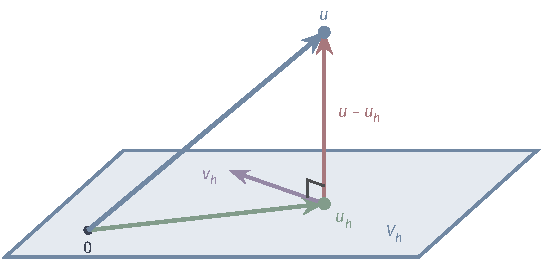
\includegraphics[width=92mm]{figures/06-differential-equations/02-partial-differential-equations/tikz/pdenum-galerkin-projection/figure.pdf}
 \caption{$a$对称正定时的Galerkin方法。真解$u$（蓝）不在有限维子空间$V_h$（浅蓝平面）中，$u_h$（绿）是它关于内积$a(\cdot,\cdot)$的正交投影，误差$u-u_h$（红）与$V_h$中的每个$v_h$（紫）都$a$-正交。}
 \label{fig:pdenum-galerkin-projection}
\end{BookInlineFigure}

\paragraph{非齐次Dirichlet数据}
上面的讨论要求试探函数和测试函数在同一个线性空间里，而边值$u=g\ne0$的函数不构成线性空间。第~\ref{chap:elliptic-equations}章的办法是作边界提升：取任何满足边值的函数$u_g$，令$w=u-u_g$，$w$就是齐次的，方程变成
\begin{equation}
 a(w,v)=\ell(v)-a(u_g,v)\qquad\text{对所有}\ v\in V .
 \label{eq:pdenum-lifted}
\end{equation}

离散时同样要做这一步，右端多出的$-a(u_g,v_h)$不能丢。在节点基下，自然的提升是用边界节点对应的基函数：$u_g=\sum_{p\in\text{边界}}g_p\varphi_p$。把基函数按内部节点I和边界节点B分块，式~\eqref{eq:pdenum-lifted}变成
\begin{equation}
 \bm{K}_{\mathrm{II}}\bm{c}_{\mathrm{I}}=\bm{b}_{\mathrm{I}}-\bm{K}_{\mathrm{IB}}\bm{g}_{\mathrm{B}} .
 \label{eq:pdenum-lifted-system}
\end{equation}

只删除边界节点的行和列，而不把$\bm{K}_{\mathrm{IB}}\bm{g}_{\mathrm{B}}$移到右端，等于把边值改成了零。对例子~\eqref{eq:pdenum-model}，下一小节将算出，正确的系统给出$(0.9571,1.5,1.4571)$，而漏掉这一项给出$(0.7071,1,0.7071)$，那是边值全为零的问题的解，如图~\ref{fig:pdenum-boundary-deletion}所示。

\begin{BookInlineFigure}
 \centering
 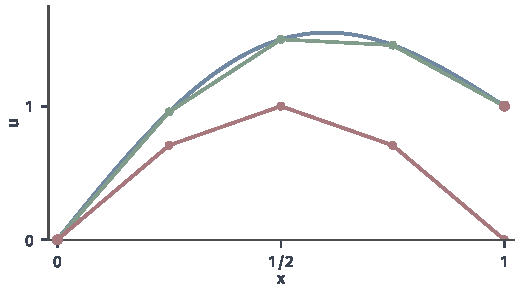
\includegraphics[width=88mm]{figures/06-differential-equations/02-partial-differential-equations/matplotlib/pdenum-boundary-deletion/figure.pdf}
 \caption{$h=1/4$的有限元解。蓝线是真解，红色大点是边值。绿线按式~\eqref{eq:pdenum-lifted-system}处理，节点值落在真解上。红线只删除了边界行和列，右端没有边值的贡献，解的右端回到了$0$。}
 \label{fig:pdenum-boundary-deletion}
\end{BookInlineFigure}

Neumann和Robin条件与此不同。它们是自然边界条件，在弱形式中通过$\ell$和$a$的边界项进入，不需要提升。

\subsection{基函数与组装}
\label{sec:pdenum-assembly}

\paragraph{主要思想}
基函数的选择决定矩阵的结构。若每个$\varphi_i$只在一小块区域上非零，那么$K_{ij}$只在$\varphi_i$和$\varphi_j$的支撑相交时非零，矩阵就是稀疏的。

在区间上取节点$0=x_0<x_1<\cdots<x_n=1$，$\varphi_i$是在$x_i$处为$1$、在其他节点处为$0$、每段上线性的\term{帽函数}（hat function）。这样的$u_h=\sum_ic_i\varphi_i$是连续的折线，且$c_i=u_h(x_i)$。

要算$K_{ij}=\int_0^1\varphi_j'\varphi_i'\,\mathrm{d}x$。帽函数的导数是分段常数，图~\ref{fig:pdenum-hat-derivatives}说明只有相邻的两个基函数才有重叠。

\begin{BookInlineFigure}
 \centering
 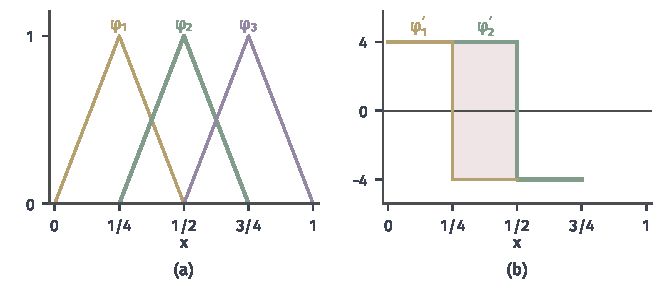
\includegraphics[width=112mm]{figures/06-differential-equations/02-partial-differential-equations/matplotlib/pdenum-hat-derivatives/figure.pdf}
 \caption{$h=1/4$的帽函数。(a)$\varphi_1,\varphi_2,\varphi_3$，相邻的帽函数才有公共支撑。(b)导数是分段常数，浅红区间是$\varphi_1'$（黄）与$\varphi_2'$（绿）唯一同时非零的区间，其上乘积为$-16$，积分得$K_{12}=-4$。}
 \label{fig:pdenum-hat-derivatives}
\end{BookInlineFigure}

每个积分都可以拆成单元上的积分之和，这把计算组织成了逐单元的循环。对单元$e=[x_{p},x_{q}]$，长度$h_e$，单元上只有$\varphi_p$和$\varphi_q$非零，它们的导数是$\mp1/h_e$，所以$2\times2$的\term{单元刚度矩阵}（element stiffness matrix）和单元载荷向量是
\begin{equation}
 \bm{k}^{e}=\frac{1}{h_e}\begin{bmatrix}1&-1\\-1&1\end{bmatrix},\qquad
 \bm{b}^{e}=\begin{bmatrix}\int_ef\varphi_p\,\mathrm{d}x\\\int_ef\varphi_q\,\mathrm{d}x\end{bmatrix}.
 \label{eq:pdenum-element-matrix}
\end{equation}
把它们按全局编号$p,q$累加到$\bm{K}$和$\bm{b}$中，这个过程称为\term{组装}（assembly）。

\needspace{6\baselineskip}
\paragraph{变量}
\begin{itemize}
 \item 节点数组$x_0,\ldots,x_n$，单元表：第$e$个单元的两个全局节点编号$(p_e,q_e)$。
 \item $\bm{K}\in\mathbb{R}^{(n+1)\times(n+1)}$：全局稀疏矩阵；$\bm{b}\in\mathbb{R}^{n+1}$：全局载荷。
 \item $\bm{k}^{e}\in\mathbb{R}^{2\times2}$，$\bm{b}^{e}\in\mathbb{R}^2$：当前单元的贡献。
\end{itemize}

\paragraph{初始化}
令$\bm{K}=\bm{0}$，$\bm{b}=\bm{0}$。例中$n=4$，$h_e=1/4$，$f=\pi^2\sin(\pi x)$，单元表为$(0,1),(1,2),(2,3),(3,4)$，节点从$0$编号。

\needspace{6\baselineskip}
\paragraph{每轮更新}
对每个单元执行下面三步，全部单元处理完后结束组装。
\begin{enumerate}
 \item 由式~\eqref{eq:pdenum-element-matrix}算出$\bm{k}^{e}$和$\bm{b}^{e}$。例中四个单元的$\bm{k}^{e}$相同，$1/h_e=4$。载荷用精确积分，四个单元依次是
 \[
  \begin{aligned}
  \bm{b}^{1}&=(0.3132,\,0.6070)^\top, & \bm{b}^{2}&=(1.0499,\,1.1716)^\top,\\
  \bm{b}^{3}&=(1.1716,\,1.0499)^\top, & \bm{b}^{4}&=(0.6070,\,0.3132)^\top.
  \end{aligned}
 \]
 \item 把$\bm{k}^{e}$加到$\bm{K}$的行列$(p_e,q_e)$上。例中第一轮后节点$0,1$构成的块是$4$乘以图~\ref{fig:pdenum-assembly}(a)的元素；第二轮再加到节点$1,2$的行列上，节点$1$的对角元变成$4+4=8$。图~\ref{fig:pdenum-assembly}是四轮的累加过程。
 \item 把$\bm{b}^{e}$加到$\bm{b}$的$p_e,q_e$分量上。例中内部节点的载荷累积成
 \[
  b_1=0.6070+1.0499=1.6569,\quad b_2=2\times1.1716=2.3431,\quad b_3=1.6569.
 \]
\end{enumerate}

\begin{BookInlineFigure}
 \centering
 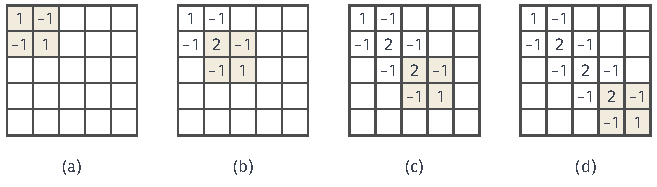
\includegraphics[width=112mm]{figures/06-differential-equations/02-partial-differential-equations/tikz/pdenum-assembly/figure.pdf}
 \caption{$n=4$的刚度矩阵（以$1/h$为单位）累加四个单元的贡献。(a)—(d)依次是加入第$1$到第$4$个单元后的结果，黄底是这一轮新加入的位置，重叠处的$1+1=2$来自相邻单元共享节点。方格是矩阵元素。}
 \label{fig:pdenum-assembly}
\end{BookInlineFigure}

组装结束后处理边值。例中$u(0)=0$、$u(1)=1$，节点$3$与边界节点$4$的耦合是$K_{34}=-4$。按式~\eqref{eq:pdenum-lifted-system}，$-K_{34}g_4=+4$加在第三个方程上，内部系统为
\[
 4\begin{bmatrix}2&-1&0\\-1&2&-1\\0&-1&2\end{bmatrix}\bm{c}
 =\begin{bmatrix}1.6569\\2.3431\\5.6569\end{bmatrix}.
\]
用式~\eqref{eq:pdenum-thomas-forward}和式~\eqref{eq:pdenum-thomas-back}解这个三对角方程，最终得到
\[
 \bm{c}=(0.9571,\,1.5000,\,1.4571)^\top .
\]

这三个数正好是真解的节点值，这不是巧合。

\paragraph{节点精确性}
节点上没有误差，是因为此时节点处的Green函数恰好落在$V_h$里。

\begin{theorem}[一维节点精确]
 \label{thm:pdenum-nodal-exact}
 设$a(u,v)=\int_0^1u'v'\,\mathrm{d}x$，$V=H^1_0(0,1)$，$V_h$是任意网格上的分片线性函数空间，$u_h$是载荷精确积分的Galerkin解。则$u_h(x_i)=u(x_i)$对所有节点成立。
\end{theorem}

\begin{proof}
 固定内部节点$x_i$，取Green函数$G_i$：它在$[0,x_i]$和$[x_i,1]$上都是线性函数，$G_i(0)=G_i(1)=0$，且$a(w,G_i)=w(x_i)$对所有$w\in V$成立。$G_i$只在$x_i$处有折角，所以$G_i\in V_h$。

 在Galerkin正交性~\eqref{eq:pdenum-orthogonality}中取$v_h=G_i$，得
 \[
  u(x_i)-u_h(x_i)=a(u-u_h,G_i)=0 .
 \]
\end{proof}

这是一维常系数问题的特殊性质。二维的Green函数在节点处奇异，变系数问题的Green函数在单元内也不是线性的，节点精确都不再成立。

它却让载荷的积分误差可以单独看出来。若单元载荷用梯形公式，则$b_i\approx hf(x_i)$，方程组除以$h$后正是差分方程~\eqref{eq:pdenum-three-point}，解就是$(0.9946,1.5530,1.4946)$。这里的误差$0.0530$完全来自数值积分。

\paragraph{高维的组装}
二维时把区域分成三角形，$\varphi_i$是在节点$i$处为$1$、在其他节点处为$0$的分片线性函数，形如金字塔，支撑是围绕节点$i$的那些三角形（图~\ref{fig:pdenum-triangle-mesh}(a)）。组装的循环完全不变，只是单元矩阵变成$3\times3$。梯度在三角形上是常向量，所以
\begin{equation}
 k^{e}_{ab}=\lvert e\rvert\,\nabla\varphi_a\cdot\nabla\varphi_b .
 \label{eq:pdenum-triangle-matrix}
\end{equation}

\begin{BookInlineFigure}
 \centering
 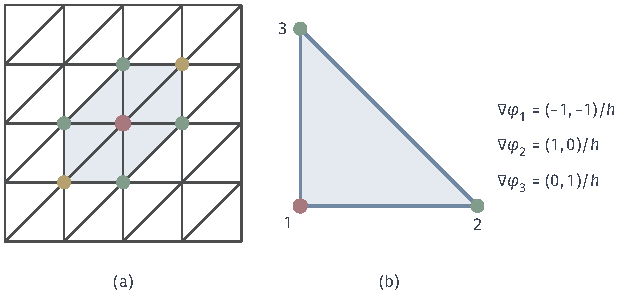
\includegraphics[width=106mm]{figures/06-differential-equations/02-partial-differential-equations/tikz/pdenum-triangle-mesh/figure.pdf}
 \caption{(a)规则三角网格，浅蓝区域是红点处基函数的支撑，由六个三角形组成，绿点和黄点是有公共单元的邻点。(b)直角边长$h$的三角形单元，三个基函数的梯度列在右侧。}
 \label{fig:pdenum-triangle-mesh}
\end{BookInlineFigure}

对图~\ref{fig:pdenum-triangle-mesh}(b)的直角三角形，$\lvert e\rvert=h^2/2$，由式~\eqref{eq:pdenum-triangle-matrix}得
\[
 \bm{k}^{e}=\frac12\begin{bmatrix}2&-1&-1\\-1&1&0\\-1&0&1\end{bmatrix}.
\]
$h$约掉了，二维的刚度矩阵元素与单元大小无关。

把中心节点周围六个三角形的贡献加起来。两个三角形的直角顶点在中心，各贡献$1$，另外四个三角形的中心节点在锐角顶点，各贡献$1/2$，对角元是$4$。四个水平、竖直邻点的边各被两个三角形共享，每个贡献$-1/2$，非对角元是$-1$；两个黄色邻点对应的矩阵元是$0$。这正是五点公式~\eqref{eq:pdenum-five-point}的模板。有限元的好处是，不规则的网格也可以用同样的循环组装。

\paragraph{各自保留的误差来源}
实际计算与上面的理想情形还有三处不同。载荷和变系数的积分通常用数值积分代替，这时解的是一个扰动后的方程，它的误差不包含在下一小节的估计里。

边界弯曲时，多边形网格覆盖的区域与真实区域不同，$V_h$可能不再是$V$的子空间，协调性被破坏，需要曲边单元或额外的分析。最后，线性方程组是用有限精度算出来的，残差不为零，Galerkin正交性也只是近似成立。

\subsection{逼近误差}
\label{sec:pdenum-fem-error}

$u_h$离$u$有多远？回答分成两步，第一步把问题化成纯粹的逼近问题，第二步才用到网格和解的光滑性。

\begin{theorem}[Céa估计]
 \label{thm:pdenum-cea}
 设$a$在$V$上有界且强制，常数分别为$M$和$\alpha$，$V_h\subset V$，$u$和$u_h$分别满足式~\eqref{eq:pdenum-weak}和式~\eqref{eq:pdenum-galerkin}。则
 \begin{equation}
  \lVert u-u_h\rVert_V\leq\frac{M}{\alpha}\inf_{v_h\in V_h}\lVert u-v_h\rVert_V .
  \label{eq:pdenum-cea}
 \end{equation}
\end{theorem}

\begin{proof}
 记$e=u-u_h$，取任意$v_h\in V_h$。由强制性，
 \[
  \alpha\lVert e\rVert_V^2\leq a(e,e) .
 \]
 把第二个$e$写成$(u-v_h)+(v_h-u_h)$，其中$v_h-u_h\in V_h$，由式~\eqref{eq:pdenum-orthogonality}，这一部分的贡献为零：
 \[
  a(e,e)=a(e,u-v_h) .
 \]
 由有界性，
 \[
  a(e,u-v_h)\leq M\lVert e\rVert_V\lVert u-v_h\rVert_V .
 \]
 三式相连，约去$\lVert e\rVert_V$（$e=0$时结论已成立），再对$v_h$取下确界。
\end{proof}

三个条件各有作用。有界性和强制性给出常数比$M/\alpha$，它描述问题的条件好坏；协调性让Galerkin正交性可用。$a$对称时，在能量范数$\lVert v\rVert_a=a(v,v)^{1/2}$下常数是$1$，$u_h$就是能量范数下的最佳逼近。

定理只说$u_h$不比$V_h$中最好的函数差多少。第二步要估计$V_h$的逼近能力，常用的办法是取节点插值$I_hu$作为具体的候选。

\begin{lemma}[分片线性插值误差]
 \label{lem:pdenum-interpolation}
 设$u\in H^2(0,1)$，$I_hu$是$u$在最大步长为$h$的网格上的分片线性插值，则
 \begin{equation}
  \lVert(u-I_hu)'\rVert_{L^2}\leq\frac{h}{\pi}\lVert u''\rVert_{L^2} .
  \label{eq:pdenum-interpolation}
 \end{equation}
\end{lemma}

\begin{proof}
 在一个单元$[a,b]$上，长度$\ell\leq h$，记$e=u-I_hu$。$e(a)=e(b)=0$，所以$\int_a^be'\,\mathrm{d}x=0$，即$e'$的平均为零。

 把$e'$按余弦函数$\cos(k\pi(x-a)/\ell)$展开，平均为零使$k=0$的项消失，系数记为$c_k$。由Parseval恒等式，
 \[
  \int_a^b(e')^2\,\mathrm{d}x=\frac{\ell}{2}\sum_{k\geq1}c_k^2\leq\frac{\ell^2}{\pi^2}\cdot\frac{\ell}{2}\sum_{k\geq1}\Bigl(\frac{k\pi}{\ell}\Bigr)^2c_k^2=\frac{\ell^2}{\pi^2}\int_a^b(e'')^2\,\mathrm{d}x .
 \]
 单元内$I_hu$线性，所以$e''=u''$。对所有单元求和即得结论。
\end{proof}

合并Céa估计与引理。在一维Poisson问题上，$a$对称，常数是$1$，能量误差满足
\begin{equation}
 \lVert(u-u_h)'\rVert_{L^2}\leq\frac{h}{\pi}\lVert u''\rVert_{L^2} .
 \label{eq:pdenum-energy-rate}
\end{equation}

$L^2$范数下的误差比能量范数高一阶，这要用到对偶论证。

\begin{theorem}[$L^2$误差]
 \label{thm:pdenum-l2}
 在一维Poisson问题上，若$u\in H^2(0,1)$，则
 \begin{equation}
  \lVert u-u_h\rVert_{L^2}\leq\frac{h}{\pi}\lVert(u-u_h)'\rVert_{L^2}\leq\frac{h^2}{\pi^2}\lVert u''\rVert_{L^2} .
  \label{eq:pdenum-l2-rate}
 \end{equation}
\end{theorem}

\begin{proof}
 记$e=u-u_h$，$z$是对偶问题$-z''=e$，$z(0)=z(1)=0$的解，$z\in H^2$且$\lVert z''\rVert_{L^2}=\lVert e\rVert_{L^2}$。用$e$检验对偶问题并分部积分，
 \[
  \lVert e\rVert_{L^2}^2=a(e,z) .
 \]
 由Galerkin正交性可以减去$I_hz\in V_h$：
 \[
  a(e,z)=a(e,z-I_hz)\leq\lVert e'\rVert_{L^2}\lVert(z-I_hz)'\rVert_{L^2} .
 \]
 用引理~\ref{lem:pdenum-interpolation}估计第二个因子，并用$\lVert z''\rVert_{L^2}=\lVert e\rVert_{L^2}$，得到
 \[
  \lVert e\rVert_{L^2}^2\leq\frac{h}{\pi}\lVert e'\rVert_{L^2}\lVert e\rVert_{L^2} .
 \]
 约去$\lVert e\rVert_{L^2}$，得第一个不等式；第二个不等式由式~\eqref{eq:pdenum-energy-rate}得到。
\end{proof}

例中$\lVert u''\rVert_{L^2}=\pi^2/\sqrt2\approx6.979$。$h=1/4$时，能量误差的上界是$0.5554$，实际是$0.4985$；$L^2$误差的中间上界是$(h/\pi)\times0.4985=0.0397$，实际是$0.0393$。$h=1/8$时对应的四个数是$0.2777$、$0.2512$、$0.0100$、$0.0099$。

\paragraph{实际阶数还看什么}
式~\eqref{eq:pdenum-energy-rate}要求$u\in H^2$。把解换成$u=x^{3/4}-x$，它属于$H^1_0$，$u''$却不平方可积。由定理~\ref{thm:pdenum-nodal-exact}，这时$u_h$就是节点插值，能量误差可以用积分精确算出。图~\ref{fig:pdenum-fem-rates}(b)表明，均匀网格的观测阶只有$0.25$。

\begin{BookInlineFigure}
 \centering
 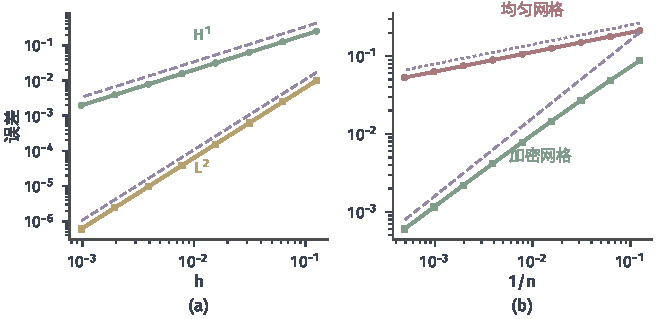
\includegraphics[width=112mm]{figures/06-differential-equations/02-partial-differential-equations/matplotlib/pdenum-fem-rates/figure.pdf}
 \caption{分片线性元的误差，紫线是参考斜率。(a)光滑解$\sin(\pi x)+x$：绿线$H^1$半范数，斜率$1$；黄线$L^2$范数，斜率$2$。(b)$u=x^{3/4}-x$的$H^1$半范数：红线是均匀网格，斜率$0.25$；绿线是向$0$加密的网格$x_i=(i/n)^4$，斜率接近$1$。}
 \label{fig:pdenum-fem-rates}
\end{BookInlineFigure}

问题集中在$x=0$附近，解的导数在那里无界。把节点按$x_i=(i/n)^4$向$0$加密后，单元数目不变，观测阶从$0.83$逐渐升到$0.94$，接近一阶。收敛阶不是方法的固有性质，它还取决于解的正则性和网格是否与之匹配。

高维的情形要结合更多因素。$k$次单元在解足够光滑、网格形状规则（三角形不退化）时，$H^1$误差是$O(h^k)$，$L^2$误差是$O(h^{k+1})$，后者还要求对偶问题具有$H^2$正则性。严格的证明需要Bramble--Hilbert引理和单元上的尺度变换，篇幅较长，读者可查阅有限元方法的专著。非凸多边形的角点附近解不属于$H^2$，均匀网格上的阶数会下降，机制与上面的一维例子相同。


\section{守恒有限体积}
\label{sec:pdenum-finite-volumes}

第~\ref{chap:scalar-conservation-laws}章的激波没有导数可言，差分公式在间断处失去依据，但有一个量即使在激波处仍然成立：任意一段区间里总量的变化，等于从两端流进流出的差。有限体积方法就以这个等式为出发点。

考虑一维标量守恒律
\begin{equation}
 \partial_tu+\partial_xF(u)=0,\qquad u(x,0)=u_0(x),
 \label{eq:pdenum-conservation-law}
\end{equation}
线性输运是$F(u)=au$的特殊情形，Burgers方程是$F(u)=u^2/2$的情形。

\subsection{单元平均与通量}
\label{sec:pdenum-cell-averages}

把$x$轴分成长度$h$的单元$C_j=[x_{j-1/2},x_{j+1/2}]$，时间步长为$\tau$。把式~\eqref{eq:pdenum-conservation-law}在$C_j\times[t_k,t_{k+1}]$上积分，$\bar{u}_j(t)$是单元平均~\eqref{eq:pdenum-cell-average}，得到一个精确的关系：
\begin{equation}
 \bar{u}_j(t_{k+1})=\bar{u}_j(t_k)-\frac{1}{h}\int_{t_k}^{t_{k+1}}\bigl(F(u_{j+1/2})-F(u_{j-1/2})\bigr)\,\mathrm{d}t ,
 \label{eq:pdenum-exact-balance}
\end{equation}
其中$u_{j\pm1/2}=u(x_{j\pm1/2},t)$。这个等式对弱解也成立，它不需要$u$可导，只需要界面上的通量有意义。

式中唯一不知道的是界面上的时间积分。用仅依赖两侧单元平均的\term{数值通量}（numerical flux）$\widehat{F}$代替它，就得到\term{守恒格式}（conservative scheme）：
\begin{equation}
 U_j^{(k+1)}=U_j^{(k)}-\lambda\Bigl(\widehat{F}_{j+1/2}^{(k)}-\widehat{F}_{j-1/2}^{(k)}\Bigr),\qquad\lambda=\frac{\tau}{h},
 \label{eq:pdenum-conservative}
\end{equation}
其中$\widehat{F}_{j+1/2}^{(k)}$是在第$j$与$j+1$单元的值$U_j^{(k)},U_{j+1}^{(k)}$处算出的数值通量。数值通量\term{相容}（consistent）是指$\widehat{F}(a,a)=F(a)$，也就是在解不变的区域里通量没有偏差。

关键的结构是：单元$j$右边的通量和单元$j+1$左边的通量是同一个数。图~\ref{fig:pdenum-fv-cells}把这件事画成了账目，从一个单元流出的量恰好流进邻居。

\begin{BookInlineFigure}
 \centering
 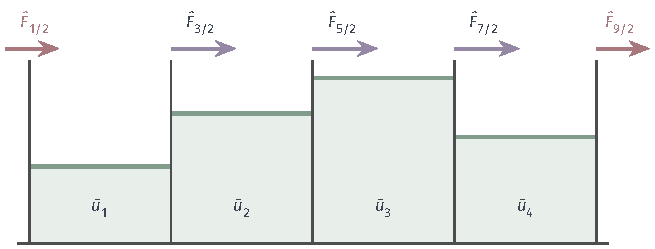
\includegraphics[width=111mm]{figures/06-differential-equations/02-partial-differential-equations/tikz/pdenum-fv-cells/figure.pdf}
 \caption{四个单元的平均值（绿）和界面通量。内部通量（紫）在左边单元中减去、在右边单元中加上，求和时抵消。总量的变化只由两端的通量（红）决定。}
 \label{fig:pdenum-fv-cells}
\end{BookInlineFigure}

把式~\eqref{eq:pdenum-conservative}对$j=1,\ldots,J$乘以$h$相加，内部的通量两两抵消，留下
\begin{equation}
 h\sum_{j=1}^JU_j^{(k+1)}=h\sum_{j=1}^JU_j^{(k)}-\tau\Bigl(\widehat{F}_{J+1/2}^{(k)}-\widehat{F}_{1/2}^{(k)}\Bigr).
 \label{eq:pdenum-telescoping}
\end{equation}
这是连续问题总量平衡的精确离散版本，不依赖$\widehat{F}$的具体形式，也不依赖$h$的大小。下面的例子说明，这个看似只是记账的性质决定了激波的速度。

\subsection{迎风与Riemann求解}
\label{sec:pdenum-upwind-riemann}

\paragraph{线性输运的迎风通量}
$F(u)=au$，设$a>0$，信息从左向右传，水流把墨水往下游带。单元界面的通量应该由上游决定，这就是\term{迎风格式}（upwind scheme）：
\begin{equation}
 \widehat{F}(U_j,U_{j+1})=aU_j .
 \label{eq:pdenum-upwind-flux}
\end{equation}
$a<0$时取$aU_{j+1}$。代入式~\eqref{eq:pdenum-conservative}，记$\mu=a\lambda$，得到更新公式
\begin{equation}
 U_j^{(k+1)}=U_j^{(k)}-\mu\bigl(U_j^{(k)}-U_{j-1}^{(k)}\bigr).
 \label{eq:pdenum-upwind}
\end{equation}

\needspace{6\baselineskip}
\paragraph{变量}
\begin{itemize}
 \item $U_j^{(k)}$：第$k$层第$j$个单元的平均，$j=1,\ldots,J$。
 \item $\widehat{F}_{j+1/2}^{(k)}$：第$j$与$j+1$单元之间的数值通量。
 \item $\mu=a\tau/h$：步长比。
\end{itemize}

\paragraph{初始化}
$U_j^{(0)}$取初值在单元上的平均。例中$a=1$，$\mu=0.5$，六个单元，方形初值的单元平均和左边界的入流状态是
\[
 \bm{U}^{(0)}=(0,\,1,\,1,\,0,\,0,\,0)^\top,\qquad U_{\text{入流}}=0 .
\]

\needspace{6\baselineskip}
\paragraph{每轮更新}
对每一层执行两步，走到$k\tau=T$结束。
\begin{enumerate}
 \item 由式~\eqref{eq:pdenum-upwind-flux}算出全部界面通量。例中第一轮，七个界面上的通量从左到右是$(0,0,1,1,0,0,0)$。
 \item 由式~\eqref{eq:pdenum-conservative}更新每个单元。例中前三轮的结果为
 \[
  \begin{aligned}
  \bm{U}^{(1)}&=(0,\,0.5,\,1,\,0.5,\,0,\,0)^\top,\\
  \bm{U}^{(2)}&=(0,\,0.25,\,0.75,\,0.75,\,0.25,\,0)^\top,\\
  \bm{U}^{(3)}&=(0,\,0.125,\,0.5,\,0.75,\,0.5,\,0.125)^\top.
  \end{aligned}
 \]
\end{enumerate}

最终各向量的分量之和都是$2$，这是式~\eqref{eq:pdenum-telescoping}的直接结果。方波被抹平了：$\mu=0.5$时每步的更新是相邻两值的平均，它和扩散有相同的作用。

\paragraph{数值黏性}
抹平的程度可以算出来。把$u$的Taylor展开代入式~\eqref{eq:pdenum-upwind}，并用方程把时间导数换成空间导数（$\partial_t^2u\approx a^2\partial_x^2u$），误差的主项给出
\begin{equation}
 \partial_tu+a\partial_xu=\nu\,\partial_x^2u+O(h^2),\qquad\nu=\frac{ah}{2}(1-\mu).
 \label{eq:pdenum-modified-equation}
\end{equation}
迎风格式更精确地求解的是一个带黏性的方程，$\nu$称为\term{数值黏性}（numerical viscosity）。它随$h\to0$消失，$\mu=1$时恰好为零，此时更新式就是整格平移。

\begin{BookInlineFigure}
 \centering
 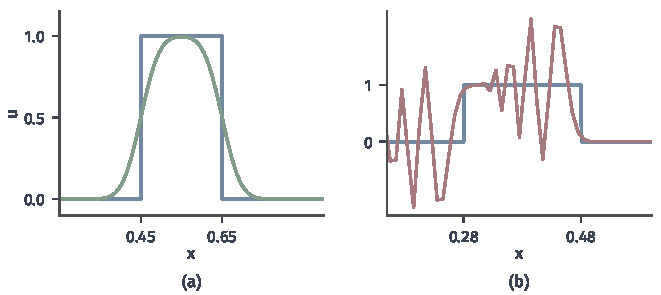
\includegraphics[width=112mm]{figures/06-differential-equations/02-partial-differential-equations/matplotlib/pdenum-upwind-smear/figure.pdf}
 \caption{$a=1$，$h=1/100$，$\mu=0.5$的方波输运。(a)$T=0.25$的迎风格式（绿）与真解（蓝），紫色虚线是修正方程~\eqref{eq:pdenum-modified-equation}的解，$\nu=0.0025$，与绿线几乎重合。(b)同样的网格用中心差分通量走到$t=0.08$（红），解已剧烈振荡。}
 \label{fig:pdenum-upwind-smear}
\end{BookInlineFigure}

图~\ref{fig:pdenum-upwind-smear}(a)中，修正方程几乎完全解释了格式的行为。(b)用的是对称的中心差分通量$\widehat{F}=a(U_j+U_{j+1})/2$，它也守恒，也相容，却不考虑信息来自哪边，第~\ref{sec:pdenum-stability}节会说明它为什么不稳定。

\paragraph{主要思想：局部Riemann问题}
Burgers方程的传播方向取决于$u$的符号，不能事先规定上游。Godunov的想法是把每个界面看作一个小的初值问题。第$k$层的单元平均是分片常数，每个界面两侧的两个常数构成一个Riemann问题，第~\ref{chap:scalar-conservation-laws}章已经解出了它的熵解。

Riemann问题的解沿界面$x=0$是一个常数，记为$u^*(U_L,U_R)$。只要各界面发出的波还没有碰到相邻界面，式~\eqref{eq:pdenum-exact-balance}中通量的时间平均就精确等于$F(u^*)$，这给出\term{Godunov格式}（Godunov scheme）的通量：
\begin{equation}
 \widehat{F}(U_L,U_R)=F\bigl(u^*(U_L,U_R)\bigr).
 \label{eq:pdenum-godunov}
\end{equation}

对凸的$F$，$u^*$可以按波的类型读出，图~\ref{fig:pdenum-riemann-fan}是两种情形。

\begin{BookInlineFigure}
 \centering
 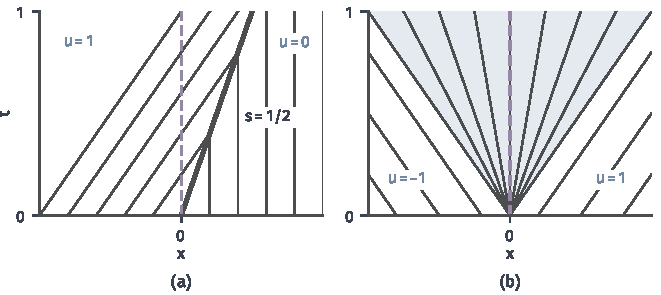
\includegraphics[width=112mm]{figures/06-differential-equations/02-partial-differential-equations/matplotlib/pdenum-riemann-fan/figure.pdf}
 \caption{Burgers方程Riemann问题的特征线（深灰），紫色虚线是界面$x=0$，Godunov通量就在这条线上读取。(a)$U_L=1$，$U_R=0$，粗线是速度$1/2$的激波，界面上的状态是$u^*=1$。(b)$U_L=-1$，$U_R=1$，浅蓝区域是稀疏波，界面上的状态是$u^*=0$。}
 \label{fig:pdenum-riemann-fan}
\end{BookInlineFigure}

$U_L\leq U_R$时解是稀疏波，$U_L>U_R$时是激波，两种情形可以合成一个公式：
\begin{equation}
 \widehat{F}(U_L,U_R)=
 \begin{cases}
 \min_{U_L\leq u\leq U_R}F(u), & U_L\leq U_R,\\
 \max_{U_R\leq u\leq U_L}F(u), & U_L>U_R .
 \end{cases}
 \label{eq:pdenum-godunov-minmax}
\end{equation}

在图~\ref{fig:pdenum-riemann-fan}(a)中，$U_L=1>U_R=0$，$u^2/2$在$[0,1]$上的最大值是$1/2$，等于$F(u^*)=F(1)$。在图(b)中，$U_L=-1<U_R=1$，$u^2/2$在$[-1,1]$上的最小值是$0$，等于$F(0)$。

\needspace{6\baselineskip}
\paragraph{变量}
\begin{itemize}
 \item $U_j^{(k)}$：第$k$层第$j$个单元的平均；$\lambda=\tau/h$。
 \item $\widehat{F}_{j+1/2}^{(k)}$：由式~\eqref{eq:pdenum-godunov-minmax}算出的界面通量。
\end{itemize}

\paragraph{初始化}
例中取Burgers方程，$\lambda=0.5$，六个单元，两端复制边界状态，也就是左边始终流入状态$1$，右边外侧始终是状态$0$：
\[
 \bm{U}^{(0)}=(1,\,1,\,1,\,0,\,0,\,0)^\top .
\]

\needspace{6\baselineskip}
\paragraph{每轮更新}
对每一层执行两步，走到$k\tau=T$结束。
\begin{enumerate}
 \item 按式~\eqref{eq:pdenum-godunov-minmax}算出全部界面通量。例中第一轮，第$3$单元及其左侧的界面通量都是$1/2$，第$3$与第$4$单元之间的状态是$(1,0)$，通量也是$1/2$，其余都是$0$。
 \item 由式~\eqref{eq:pdenum-conservative}更新。第一轮只有第$4$单元改变：
 \[
  U_4^{(1)}=0-0.5\times(0-0.5)=0.25 .
 \]
 第二轮界面$(1,0.25)$的通量仍是$1/2$，界面$(0.25,0)$的通量是$F(0.25)=0.03125$，于是
 \[
  U_4^{(2)}=0.25-0.5(0.03125-0.5)=0.4844,\qquad U_5^{(2)}=0.0156 .
 \]
 第三轮界面$(0.4844,0.0156)$的通量是$F(0.4844)=0.1173$，界面$(0.0156,0)$的通量是$0.00012$，
 \[
  \begin{gathered}
  U_4^{(3)}=0.4844+0.5(0.5-0.1173)=0.6757,\\
  U_5^{(3)}=0.0742,\qquad U_6^{(3)}=0.00006 .
  \end{gathered}
 \]
\end{enumerate}

最终各层分量之和依次是$3,\,3.25,\,3.5,\,3.75$，每步增加$\lambda\cdot\tfrac12=0.25$，也就是流入的量每步推动间断前进四分之一个单元。一个单元长$h$，一步时长$\tau$，所以间断的速度是$(h/4)/\tau=1/2$，这正是Rankine--Hugoniot条件给出的激波速度。这个速度来自式~\eqref{eq:pdenum-telescoping}，不依赖网格的细节。

\paragraph{丢掉守恒的代价}
Burgers方程的另一种写法$\partial_tu+u\partial_xu=0$在光滑解上与守恒形式等价。按它写一个迎风差分：$u\geq0$时
\[
 U_j^{(k+1)}=U_j^{(k)}-\lambda U_j^{(k)}\bigl(U_j^{(k)}-U_{j-1}^{(k)}\bigr).
\]
代入同一组初值，第$4$单元的$U_4=0$，修正项$\lambda U_4(U_4-U_3)=0$，$U_4$永远不变。数值解是定态，激波根本不动。

\begin{BookInlineFigure}
 \centering
 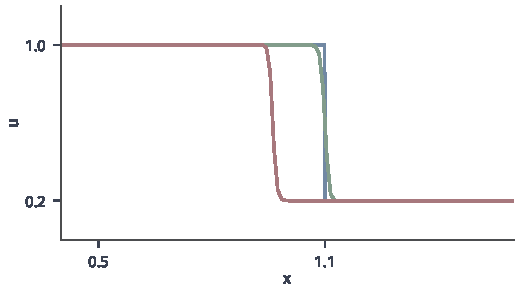
\includegraphics[width=88mm]{figures/06-differential-equations/02-partial-differential-equations/matplotlib/pdenum-godunov-shock/figure.pdf}
 \caption{Burgers方程，左状态$1$，右状态$0.2$，初始间断在$x=0.5$，$h=0.01$，$\lambda=0.5$，$T=1$。蓝线是真解，激波在$x=1.1$；绿线是Godunov格式，半高位置$1.105$；红线是非守恒的迎风差分，半高位置$0.965$，平均速度约为$0.465$，真值是$0.6$。}
 \label{fig:pdenum-godunov-shock}
\end{BookInlineFigure}

图~\ref{fig:pdenum-godunov-shock}换了一组不那么极端的数据，非守恒格式不再冻结，但速度仍然是错的。守恒的约束恰好保证了激波速度的正确，第~\ref{sec:pdenum-nonlinear}小节的定理说明这不是偶然的。

\subsection{熵选择}
\label{sec:pdenum-entropy}

守恒格式的极限若存在就是弱解，但弱解可以不唯一。第~\ref{chap:scalar-conservation-laws}章用熵条件挑出物理上的解，离散格式也需要类似的选择机制。

\paragraph{一个守恒却选错解的例子}
Godunov通量要解Riemann问题，一个省事的替代是取平均速度$s=(U_L+U_R)/2$当作波速，再按迎风法则取通量：
\begin{equation}
 \widehat{F}_{\mathrm{R}}(U_L,U_R)=
 \begin{cases}F(U_L), & s\geq0,\\F(U_R), & s<0.\end{cases}
 \label{eq:pdenum-roe}
\end{equation}
这是一种Roe型通量，它相容，代入式~\eqref{eq:pdenum-conservative}后也是守恒的。

取Burgers方程，初值在原点由$-1$跳到$1$。这时$s=0$，通量$\widehat{F}_{\mathrm{R}}=F(-1)=1/2$，它和两侧单元内部的通量相同，更新量为零。这个间断永远不动，是一个定态的膨胀激波。

它满足Rankine--Hugoniot条件，确实是弱解，只是不满足熵条件，真解是从原点展开的稀疏波。用Godunov通量走一步，$\lambda=0.5$，四个单元$(-1,-1,1,1)$的中间界面通量是$\min_{[-1,1]}F=0$，得到
\[
 U_2^{(1)}=-0.75,\qquad U_3^{(1)}=0.75,
\]
间断立即开始展开。

\begin{BookInlineFigure}
 \centering
 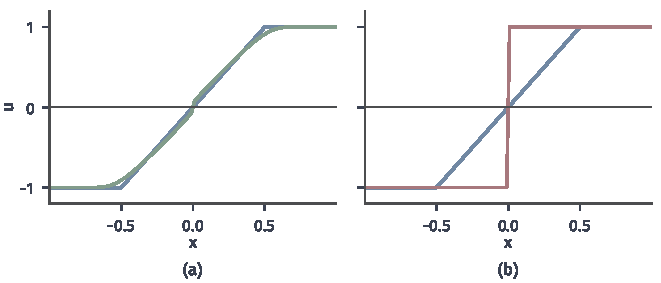
\includegraphics[width=112mm]{figures/06-differential-equations/02-partial-differential-equations/matplotlib/pdenum-entropy-fix/figure.pdf}
 \caption{Burgers方程，初值在$x=0$处由$-1$跳到$1$，$h=0.02$，$\lambda=0.5$，$T=0.5$，蓝线是熵解。(a)Godunov格式（绿）贴合稀疏波，$L^1$误差$0.047$。(b)Roe型通量（红）停留在初始的膨胀激波上，$L^1$误差$0.5$，加密网格不能改善。}
 \label{fig:pdenum-entropy-fix}
\end{BookInlineFigure}

图~\ref{fig:pdenum-entropy-fix}表明，离散守恒只负责总量，不能排除错误的间断。Roe型通量的问题出在特征速度于$U_L$和$U_R$之间变号的界面上，式~\eqref{eq:pdenum-roe}只看到了平均速度。

\paragraph{单调格式}
要选出正确的解，一个充分的结构性条件是单调。把式~\eqref{eq:pdenum-conservative}写成
\begin{equation}
 U_j^{(k+1)}=H\bigl(U_{j-1}^{(k)},U_j^{(k)},U_{j+1}^{(k)}\bigr).
 \label{eq:pdenum-scheme-h}
\end{equation}
若$H$对三个自变量都单调不减，称格式是\term{单调格式}（monotone scheme）。直观上，初值处处增大，下一层也处处增大，这和熵解的比较原理对应。

设$\widehat{F}$是Lipschitz的，对第一个变量不减，对第二个变量不增。$H$对第一、第三个变量的单调性由此直接得到，对中间变量$b$的单调性要求
\[
 \lambda\bigl(\partial_1\widehat{F}(b,c)-\partial_2\widehat{F}(a,b)\bigr)\leq1 .
\]

Godunov通量满足前两条。式~\eqref{eq:pdenum-godunov-minmax}中，增大$U_L$时，第一种情形的取最小值的区间缩小，最小值不减；第二种情形的取最大值的区间扩大，最大值不减。增大$U_R$的情形相反，通量不增。

步长条件也可以写得更具体。$\partial_1\widehat{F}(b,c)$只有$0$和$F'(b)$两种取值，后者只在$F'(b)>0$时出现；$\partial_2\widehat{F}(a,b)$同样只有$0$和$F'(b)$两种取值，后者只在$F'(b)<0$时出现。两者不会同时非零，所以条件成为
\begin{equation}
 \lambda\max\lvert F'\rvert\leq1 .
 \label{eq:pdenum-monotone-cfl}
\end{equation}

Roe型通量不单调。$U_L=-1$，$U_R=1$时通量是$1/2$；把$U_R$略微减小，$s<0$，通量变成$F(U_R)<1/2$。减小$U_R$反而减小了通量，方向与要求相反。

\paragraph{单调格式满足离散熵不等式}
对常数$c$，把$\max(a,c)$记作$a\vee c$，$\min(a,c)$记作$a\wedge c$。取Kružkov熵$\lvert u-c\rvert$，相应的熵通量是$\mathrm{sgn}(u-c)(F(u)-F(c))$。单调性足以产生这些熵不等式的离散版本。

\begin{theorem}[离散熵不等式]
 \label{thm:pdenum-discrete-entropy}
 设式~\eqref{eq:pdenum-scheme-h}的$H$单调不减，$\widehat{F}$相容。对任意常数$c$，令
 \begin{equation}
  Q_c(a,b)=\widehat{F}(a\vee c,\,b\vee c)-\widehat{F}(a\wedge c,\,b\wedge c).
  \label{eq:pdenum-entropy-flux}
 \end{equation}
 则格式的解满足
 \begin{equation}
  \begin{aligned}
  \lvert U_j^{(k+1)}-c\rvert\leq{}&\lvert U_j^{(k)}-c\rvert\\
  &-\lambda\Bigl(Q_c\bigl(U_j^{(k)},U_{j+1}^{(k)}\bigr)-Q_c\bigl(U_{j-1}^{(k)},U_j^{(k)}\bigr)\Bigr).
  \end{aligned}
  \label{eq:pdenum-discrete-entropy}
 \end{equation}
\end{theorem}

\begin{proof}
 记$a=U_{j-1}^{(k)}$，$b=U_j^{(k)}$，$d=U_{j+1}^{(k)}$。由相容性，常数状态不变，$H(c,c,c)=c$。

 由单调性，$H(a\vee c,b\vee c,d\vee c)$同时不小于$H(a,b,d)$和$H(c,c,c)=c$，所以
 \[
  H(a\vee c,b\vee c,d\vee c)\geq U_j^{(k+1)}\vee c .
 \]
 同理，
 \[
  H(a\wedge c,b\wedge c,d\wedge c)\leq U_j^{(k+1)}\wedge c .
 \]

 两式相减，并用$\lvert s-c\rvert=s\vee c-s\wedge c$，得到
 \[
  \lvert U_j^{(k+1)}-c\rvert\leq H(a\vee c,b\vee c,d\vee c)-H(a\wedge c,b\wedge c,d\wedge c) .
 \]
 代入$H$的定义，$(b\vee c)-(b\wedge c)=\lvert b-c\rvert$，通量部分合起来就是式~\eqref{eq:pdenum-entropy-flux}的差分。
\end{proof}

由相容性，$Q_c(a,a)=\mathrm{sgn}(a-c)(F(a)-F(c))$，所以$Q_c$是连续熵通量的相容逼近。这个不等式怎样传到极限，留到第~\ref{sec:pdenum-nonlinear}小节。

单调性有代价。单调格式至多是一阶精度，证明要分析格式在光滑解上的修正方程，篇幅较长，读者可查阅Harten、Hyman和Lax的原始工作。这就是单调格式总带有数值黏性的原因。

\section{稳定性与收敛}
\label{sec:pdenum-stability}

前面三种方法都用到了同一个模式：差分方程上是$\lVert\bm{A}_h^{-1}\rVert_\infty\leq1/8$，Galerkin方法上是强制常数，扩散方程上是放大因子不超过$1$。这里把这些词的含义固定下来，并说明线性问题和非线性守恒问题为什么不能共用一条判据。

\paragraph{三个概念}
比较不同网格上的解，先要选定一族离散范数。常用的有
\[
 \lVert\bm{v}\rVert_{\infty}=\max_j\lvert v_j\rvert,\qquad
 \lVert\bm{v}\rVert_{1,h}=h\sum_j\lvert v_j\rvert,\qquad
 \lVert\bm{v}\rVert_{2,h}=\Bigl(h\sum_j\lvert v_j\rvert^2\Bigr)^{1/2}.
\]
下面的概念都依赖于范数的选取，同一个格式可以在一种范数下稳定，在另一种范数下不稳定。

对线性单步格式$\bm{U}^{(k+1)}=\bm{B}_\tau\bm{U}^{(k)}$，$h$随$\tau$按固定的关系变化，三个概念的含义如下。

\begin{definition}[一致性、稳定性与收敛]
 \label{def:pdenum-consistency-stability}
 设真解充分光滑，局部误差$\bm{\eta}^{(k)}$由下式定义：
 \begin{equation}
  \bm{R}_hu(t_{k+1})=\bm{B}_\tau\bm{R}_hu(t_k)+\tau\,\bm{\eta}^{(k)} .
  \label{eq:pdenum-local-error}
 \end{equation}
 若$\max_k\lVert\bm{\eta}^{(k)}\rVert\to0$，称格式\term{一致}（consistent）。若存在$\tau_0,C_T$，使
 \begin{equation}
  \lVert\bm{B}_\tau^k\rVert\leq C_T\qquad\text{对所有}\ 0<\tau\leq\tau_0,\ k\tau\leq T,
  \label{eq:pdenum-stable}
 \end{equation}
 称格式\term{稳定}（stable）。若$k\tau\to t$时$\bm{U}^{(k)}$与$\bm{R}_hu(t)$的差趋于零，称格式收敛（convergent）。
\end{definition}

稳定性是对离散算子幂的一致界，常数$C_T$允许依赖$T$，它只描述有限时间。

\subsection{线性格式}
\label{sec:pdenum-linear}

\paragraph{一致性加稳定性}
由式~\eqref{eq:pdenum-local-error}减去格式本身，$\bm{e}^{(k)}=\bm{R}_hu(t_k)-\bm{U}^{(k)}$满足
\[
 \bm{e}^{(k+1)}=\bm{B}_\tau\bm{e}^{(k)}+\tau\bm{\eta}^{(k)} .
\]
递推展开，得到
\begin{equation}
 \bm{e}^{(k)}=\bm{B}_\tau^k\bm{e}^{(0)}+\tau\sum_{l=0}^{k-1}\bm{B}_\tau^{k-1-l}\bm{\eta}^{(l)} .
 \label{eq:pdenum-error-duhamel}
\end{equation}
用稳定性估计每个幂，得到
\begin{equation}
 \lVert\bm{e}^{(k)}\rVert\leq C_T\Bigl(\lVert\bm{e}^{(0)}\rVert+T\max_l\lVert\bm{\eta}^{(l)}\rVert\Bigr).
 \label{eq:pdenum-lax-bound}
\end{equation}
一致性保证右端趋于零，这就是收敛，收敛阶就是局部误差的阶。

反过来，收敛能否推出稳定？在恰当的框架下回答是肯定的。为了让所有网格落在同一个空间里，这里把格式看成一个Banach空间上的算子族，网格函数延拓成分片常数函数后就落入这个框架。

\begin{theorem}[Lax等价定理]
 \label{thm:pdenum-lax}
 设$X$是Banach空间，$S(t)$是适定线性初值问题的解算子，在$[0,T]$上一致有界且强连续。$B_\tau$是$X$上的有界线性算子，在稠密子集$D\subset X$上一致，即对$u_0\in D$，
 \begin{equation}
  \frac{1}{\tau}\sup_{k\tau\leq T}\bigl\lVert\bigl(B_\tau S(k\tau)-S((k+1)\tau)\bigr)u_0\bigr\rVert\to0 .
  \label{eq:pdenum-lax-consistent}
 \end{equation}
 则格式稳定，当且仅当对每个$u_0\in X$，只要$\tau\to0$且$k\tau\to t\in[0,T]$，就有$B_\tau^ku_0\to S(t)u_0$。
\end{theorem}

\begin{proof}
 先证稳定推出收敛。对$u_0\in D$，望远镜求和给出
 \[
  B_\tau^ku_0-S(k\tau)u_0=\sum_{l=0}^{k-1}B_\tau^{k-1-l}\bigl(B_\tau S(l\tau)-S((l+1)\tau)\bigr)u_0 .
 \]
 由稳定性和条件~\eqref{eq:pdenum-lax-consistent}，右端的范数不超过$C_Tk\tau$乘以一个趋于零的量。

 对一般的$u_0\in X$，用$D$中的元素逼近它。稳定性控制$B_\tau^k$作用在差上的量，$S(k\tau)$的一致有界性控制另一边，所以$B_\tau^ku_0-S(k\tau)u_0\to0$。再由强连续性，$S(k\tau)u_0\to S(t)u_0$。

 再证收敛推出稳定。假设格式不稳定，则存在$\tau_n\to0$和$k_n$，$k_n\tau_n\leq T$，使$\lVert B_{\tau_n}^{k_n}\rVert\to\infty$。取子序列使$k_n\tau_n\to t$。对每个$u_0\in X$，收敛性说明序列$B_{\tau_n}^{k_n}u_0$收敛，因而有界。由一致有界原理，$\sup_n\lVert B_{\tau_n}^{k_n}\rVert<\infty$，矛盾。
\end{proof}

定理的前提不可省略：问题必须线性且适定，格式必须线性，收敛要对$X$中每一个初值成立。

\paragraph{扩散格式的稳定估计}
显式Euler方法的稳定性可以用两种范数验证。在$\lVert\cdot\rVert_{2,h}$下，$\bm{I}-\tau\bm{A}_h$对称，特征值是$1-\tau\lambda_m$，所以范数不超过$1$的条件正是式~\eqref{eq:pdenum-ftcs-stability}，此时$C_T=1$。

在$\lVert\cdot\rVert_\infty$下，$r\leq1/2$时，式~\eqref{eq:pdenum-ftcs-component}可以写成
\[
 U_j^{(k+1)}=(1-2r)U_j^{(k)}+rU_{j-1}^{(k)}+rU_{j+1}^{(k)},
\]
三个系数非负且和为$1$，新值是旧值的凸组合，于是
\[
 \lVert\bm{U}^{(k+1)}\rVert_\infty\leq\lVert\bm{U}^{(k)}\rVert_\infty .
\]
这是热的抹平在离散层面上的体现。

\paragraph{Fourier稳定性分析}
规则网格、常系数、周期边界（或全直线）的情形，离散Fourier变换把格式对角化。把模式$U_j=\mathrm{e}^{\mathrm{i}j\xi}$代入格式，$\xi\in[-\pi,\pi]$，每步乘上一个放大因子$g(\xi)$。由Parseval恒等式，
\begin{equation}
 \lVert\bm{B}_\tau^k\rVert_{2,h}=\max_\xi\lvert g(\xi)\rvert^k .
 \label{eq:pdenum-von-neumann}
\end{equation}
稳定的充要条件是存在$C$，使$\lvert g(\xi)\rvert\leq1+C\tau$对所有$\xi$成立。

扩散格式~\eqref{eq:pdenum-ftcs-component}的放大因子是
\[
 g(\xi)=1+r(\mathrm{e}^{-\mathrm{i}\xi}-2+\mathrm{e}^{\mathrm{i}\xi})=1-4r\sin^2\frac{\xi}{2} .
\]
它在$\xi=\pi$时取到最小值$1-4r$，$\lvert g\rvert\leq1$的条件是$r\leq1/2$，与上面的结论一致。

迎风格式~\eqref{eq:pdenum-upwind}的放大因子$g(\xi)=1-\mu(1-\mathrm{e}^{-\mathrm{i}\xi})$在复平面上是以$1-\mu$为心、半径$\mu$的圆，并且
\begin{equation}
 \lvert g(\xi)\rvert^2=1-4\mu(1-\mu)\sin^2\frac{\xi}{2} .
 \label{eq:pdenum-upwind-factor}
\end{equation}
所以$0\leq\mu\leq1$时稳定。中心差分通量的放大因子是$g(\xi)=1-\mathrm{i}\mu\sin\xi$，$\lvert g\rvert^2=1+\mu^2\sin^2\xi$，对固定的$\mu>0$都大于$1$（$\sin\xi=0$处除外），这就是图~\ref{fig:pdenum-upwind-smear}(b)中振荡的来源。图~\ref{fig:pdenum-fourier-factors}把这三种情形画在复平面上，轨迹跑出单位圆的部分就是被放大的模式。

\begin{BookInlineFigure}
 \centering
 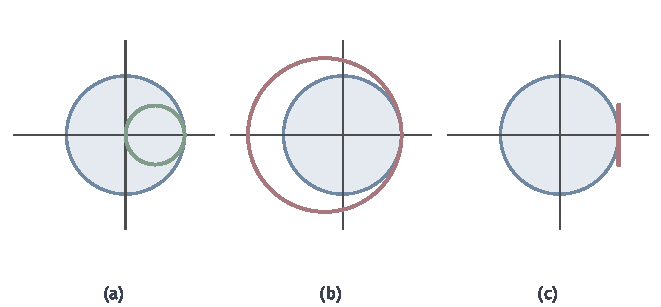
\includegraphics[width=112mm]{figures/06-differential-equations/02-partial-differential-equations/matplotlib/pdenum-fourier-factors/figure.pdf}
 \caption{输运格式的放大因子$g(\xi)$在复平面上的轨迹，浅蓝圆盘是$\lvert g\rvert\leq1$。(a)迎风格式$\mu=0.5$（绿），轨迹在圆盘内。(b)迎风格式$\mu=1.3$（红），最大模$1.6$，大部分在圆盘外。(c)中心差分$\mu=0.5$（红），轨迹是一段竖直线段，只在切点处不在圆外，最大模约为$1.118$。}
 \label{fig:pdenum-fourier-factors}
\end{BookInlineFigure}

\paragraph{边界闭合要单独检查}
Fourier分析的前提是周期边界或全直线，真实问题的边界不属于这个情形。边界的处理可能破坏内部的稳定性。

对$(0,1)$上的热方程，左端加上散热边界$\partial_xu(0,t)=\beta u(0,t)$，$\beta>0$，这个条件在物理上是耗散的。用虚拟节点$U_{-1}$和中心差分$(U_1-U_{-1})/(2h)=\beta U_0$消去虚拟节点，边界节点的更新是
\begin{equation}
 U_0^{(k+1)}=\bigl(1-2r(1+\beta h)\bigr)U_0^{(k)}+2rU_1^{(k)} .
 \label{eq:pdenum-robin-closure}
\end{equation}

系数非负的条件是$r\leq1/(2+2\beta h)$，比内部条件$r\leq1/2$更严。取$h=1/20$，$\beta=20$，$r=0.45$，内部的Fourier条件满足，边界节点的系数却是$-0.8$，迭代矩阵的谱半径是$1.173$，结果见图~\ref{fig:pdenum-boundary-closure}。

\begin{BookInlineFigure}
 \centering
 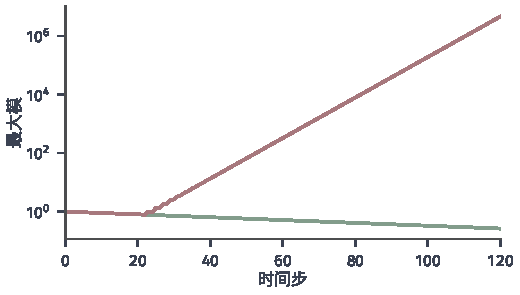
\includegraphics[width=88mm]{figures/06-differential-equations/02-partial-differential-equations/matplotlib/pdenum-boundary-closure/figure.pdf}
 \caption{显式格式解热方程的最大模随时间步的变化，$h=1/20$，$r=0.45$，右端$u=0$。绿线是左端Dirichlet条件，谱半径$0.990$，解衰减。红线是左端的散热条件~\eqref{eq:pdenum-robin-closure}，$\beta=20$，谱半径$1.173$，内部完全相同的格式发生指数增长。}
 \label{fig:pdenum-boundary-closure}
\end{BookInlineFigure}

反过来，只看矩阵的特征值也可能误判。对迎风格式取$\mu=1.5$，入流边界取零，矩阵是下双对角矩阵，特征值全是$-0.5$，谱半径小于$1$。可是这个矩阵远非正规，$N=20$时$\lVert\bm{B}^k\rVert_2$在$k=1,5,10,20$上依次约为$2.0$、$31.5$、$982$、$8.0\times10^5$，暂态增长足以毁掉计算。

\subsection{CFL条件}
\label{sec:pdenum-cfl}

上面得到的$\mu\leq1$有一个不依赖放大因子的解释：数值解必须能够看到它应该看到的初值。

\paragraph{依赖区域的比较}
对$\partial_tu+a\partial_xu=0$，$a>0$，点$(x_j,t_k)$的解等于初值在特征线足点$x_j-at_k$处的值（第~\ref{chap:transport-equations}章）。迎风格式每走一步只向左多看一个单元，所以$U_j^{(k)}$依赖的初值位于$[x_j-kh,x_j]$。

足点的距离是$at_k=\mu kh$，要落在这个区间内，就要$\mu\leq1$。图~\ref{fig:pdenum-cfl-domains}是两种情形的对比。

\begin{BookInlineFigure}
 \centering
 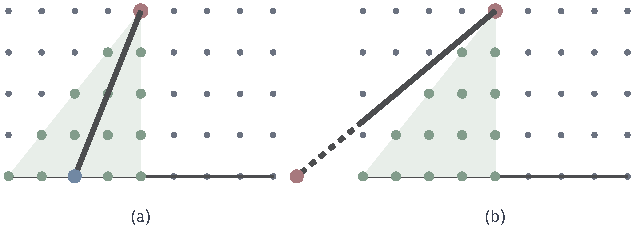
\includegraphics[width=107mm]{figures/06-differential-equations/02-partial-differential-equations/tikz/pdenum-cfl-domains/figure.pdf}
 \caption{迎风格式的依赖区域，顶部红点是要计算的值，绿点和浅绿三角形是它依赖的网格点，粗线是过红点的特征线。(a)$\mu=0.5$，足点（蓝）在依赖区域内。(b)$\mu=1.5$，特征线从依赖区域左侧穿出，足点（红）落在格式看不到的地方。}
 \label{fig:pdenum-cfl-domains}
\end{BookInlineFigure}

\begin{theorem}[CFL条件的必要性]
 \label{thm:pdenum-cfl}
 考虑$\partial_tu+a\partial_xu=0$的显式格式，步长比$\mu=a\tau/h$固定，单步模板向上游最多延伸$m$个单元。若$\mu>m$，则格式不可能对所有连续的初值收敛。
\end{theorem}

\begin{proof}
 固定$(x,t)$，$t>0$。$k\tau=t$时，$U_j^{(k)}$只依赖距$x_j$不超过$mkh$的上游初值，而
 \[
  mkh=m\,t\,\frac{h}{\tau}=\frac{m}{\mu}\,at<at .
 \]
 所以足点$x-at$与依赖区域之间有一段固定的距离。

 取一个在依赖区域内为零、在足点处非零的连续初值$u_0$。数值解在所有网格上都恒为零，而真解是$u_0(x-at)\ne0$，所以不收敛。
\end{proof}

这个条件称为\term{CFL条件}（Courant--Friedrichs--Lewy condition）。定理说的是必要性，反过来不成立：中心差分格式在$\mu\leq1$时满足CFL条件，但放大因子大于$1$，并不稳定。依赖区域够大只说明格式有可能拿到正确信息，这些信息是否被正确使用，还要看更新系数和边界处理。

$\mu=1.5$时，迎风格式对初值$(0,1,0,0)$走一步是$(0,-0.5,1.5,0)$，第二步是$(0,0.25,-1.5,2.25)$，最大模每步放大$1.5$倍。

用同样的比较看其他情形。隐式格式的依赖区域是整个网格，CFL条件自动满足，但这不等于大步长下精度也好。Burgers方程的特征速度依赖解，条件成为$\lambda\max\lvert u\rvert\leq1$，与式~\eqref{eq:pdenum-monotone-cfl}吻合。

热方程的显式格式的依赖区域宽度是$2kh=2t\,h/\tau$，连续问题的依赖区域是整条线，要填满它只需$h/\tau\to\infty$。$\tau\sim h^2$自然满足这一点，可见$r\leq1/2$这个限制并不是CFL条件，它更严格，来自稳定性。

\subsection{非线性守恒格式}
\label{sec:pdenum-nonlinear}

Lax等价定理依赖线性：误差传播写成了$\bm{B}_\tau$的幂。非线性守恒律的解甚至会在有限时间产生间断，因此要换一条路线，把“极限是什么”和“是否收敛”分开回答。

\begin{theorem}[Lax--Wendroff定理]
 \label{thm:pdenum-lax-wendroff}
 设$\widehat{F}$相容且局部Lipschitz，$\lambda=\tau/h$固定，$U^{(h)}(x,t)$是式~\eqref{eq:pdenum-conservative}的解构成的分片常数函数，初值取$u_0\in L^\infty(\mathbb{R})$的单元平均。若$h\to0$时$U^{(h)}$一致有界，且在$L^1_{\mathrm{loc}}$中收敛到$u$，则$u$是式~\eqref{eq:pdenum-conservation-law}的弱解，即对每个$\phi\in C_c^\infty(\mathbb{R}\times[0,T))$，
 \begin{equation}
  \int_0^T\!\!\int_{\mathbb{R}}\bigl(u\,\partial_t\phi+F(u)\,\partial_x\phi\bigr)\,\mathrm{d}x\,\mathrm{d}t+\int_{\mathbb{R}}u_0\,\phi(x,0)\,\mathrm{d}x=0 .
  \label{eq:pdenum-lw-limit}
 \end{equation}
\end{theorem}

\begin{proof}
 记$\phi_j^{(k)}=\phi(x_j,t_k)$。把式~\eqref{eq:pdenum-conservative}乘以$h\phi_j^{(k)}$，对$j,k$求和，再在时间和空间上分别作Abel求和，把差分转到$\phi$上。$\phi$有紧支集，没有边界项，得到
 \[
  \begin{aligned}
  &h\sum_jU_j^{(0)}\phi_j^{(0)}
  +h\tau\sum_{k\geq1}\sum_jU_j^{(k)}\frac{\phi_j^{(k)}-\phi_j^{(k-1)}}{\tau}\\
  &\qquad+h\tau\sum_{k\geq0}\sum_j\widehat{F}_{j+1/2}^{(k)}\frac{\phi_{j+1}^{(k)}-\phi_j^{(k)}}{h}=0 .
  \end{aligned}
 \]

 第一项趋于$\int u_0\phi(x,0)\,\mathrm{d}x$，因为$U_j^{(0)}$是单元平均。第二项中差商一致趋于$\partial_t\phi$，又有$U^{(h)}\to u$，所以它趋于$\iint u\,\partial_t\phi$。

 第三项要用相容性。把$\widehat{F}_{j+1/2}^{(k)}$换成$F(U_j^{(k)})=\widehat{F}(U_j^{(k)},U_j^{(k)})$，由Lipschitz性质，代价不超过常数乘以
 \[
  h\tau\sum_{k,j}\lvert U_{j+1}^{(k)}-U_j^{(k)}\rvert ,
 \]
 求和只在$\phi$的支集附近进行。这个量是$U^{(h)}$平移$h$前后之差的$L^1$范数，由$U^{(h)}$在$L^1_{\mathrm{loc}}$中收敛和平移的连续性，它趋于零。余下的部分趋于$\iint F(u)\,\partial_x\phi$，这里用到$F$的局部Lipschitz性和一致有界性。
\end{proof}

定理的假设里已经包含了收敛，它只回答极限是什么，也没有说是哪一个弱解。图~\ref{fig:pdenum-entropy-fix}(b)的Roe型通量相容又守恒，数值解收敛到的是膨胀激波这个错误的弱解。

要得到熵解，需要把定理~\ref{thm:pdenum-discrete-entropy}的不等式传到极限。对$\phi\geq0$作与上面相同的Abel求和，不等式保持方向，极限给出
\begin{equation}
 \begin{gathered}
 \iint\bigl(\lvert u-c\rvert\,\partial_t\phi+\mathrm{sgn}(u-c)(F(u)-F(c))\,\partial_x\phi\bigr)\,\mathrm{d}x\,\mathrm{d}t\\
 +\int\lvert u_0-c\rvert\,\phi(x,0)\,\mathrm{d}x\geq0 .
 \end{gathered}
 \label{eq:pdenum-entropy-limit}
\end{equation}
这对每个常数$c$成立，正是第~\ref{chap:scalar-conservation-laws}章的Kružkov熵条件，满足它的解是唯一的。

余下的问题是收敛本身。单调格式的解不超出初值的上下界，这是单调性和常数状态不变的直接推论。全变差也不增加，由Helly选择定理可得$L^1_{\mathrm{loc}}$中收敛的子序列；全变差不增的证明需要Crandall--Tartar引理，篇幅较长，读者可查阅守恒律数值方法的专著。子序列的极限都是唯一的熵解，所以整个序列收敛。

表~\ref{tab:pdenum-linear-nonlinear}对比两种论证。三件事分别对应三个不同的工具，少了哪一个都不够。

\begin{BookInlineTable}
 \centering
 \caption{线性问题与非线性守恒律的收敛论证。}
 \label{tab:pdenum-linear-nonlinear}
 \begin{tabular}{p{20mm}p{34mm}p{40mm}}
  \toprule
  要回答的问题 & 线性格式 & 非线性守恒格式\\
  \midrule
  是否收敛 & 一致性加稳定性（Lax等价） & 有界性加全变差控制给出紧性\\
  极限是什么 & 自动是原问题的解 & 守恒且相容（Lax--Wendroff）\\
  选出哪个解 & 解唯一，无须选择 & 离散熵不等式（单调格式）\\
  误差的范数 & $\lVert\cdot\rVert_{2,h}$等 & 通常是$L^1_{\mathrm{loc}}$，间断处不用最大模\\
  \bottomrule
 \end{tabular}
\end{BookInlineTable}

收敛速度也不同。图~\ref{fig:pdenum-godunov-shock}的激波问题在$T=0.8$时，单元数取$40$、$80$、$160$、$320$、$640$，$L^1$误差依次为
\[
 0.0300,\quad 0.0144,\quad 0.0079,\quad 0.0035,\quad 0.0019,
\]
观测阶略有起伏，整体接近$1$。

\section{误差与计算成本}
\label{sec:pdenum-error-cost}

一次计算结束后，怎样判断结果有多可信，又该把算力花在哪里？式~\eqref{eq:pdenum-error-split}把总误差分成了几段，这里逐段检验，再比较各种做法的代价。

\paragraph{用加密检查实际收敛}
真解已知时，比较相邻两层网格的误差，就得到\term{观测阶}（observed order）：
\begin{equation}
 p_{\mathrm{obs}}=\log_2\frac{E(h)}{E(h/2)} .
 \label{eq:pdenum-observed-order}
\end{equation}
表~\ref{tab:pdenum-fd-refine}和图~\ref{fig:pdenum-fd-rates}都是这样读出阶数的。真解未知时，有两种常用的办法。

第一种是构造解：先选一个光滑函数当作解，代入方程算出对应的源项和边值，再用这些数据检验程序。式~\eqref{eq:pdenum-model}就是这样得到的。这种办法检验的是程序和格式，不检验实际问题的解是否足够光滑。

第二种是比较三层网格。若误差的主项是$Ch^p$，相邻两层解的差的比值给出
\begin{equation}
 p_{\mathrm{obs}}\approx\log_2\frac{\lVert\bm{U}_h-\bm{U}_{h/2}\rVert}{\lVert\bm{U}_{h/2}-\bm{U}_{h/4}\rVert},
 \label{eq:pdenum-three-grid}
\end{equation}
这里的差要在公共节点上计算。它的前提是这几层网格已进入渐近范围，解的奇性、激波和未分辨的小尺度都可能破坏这一点。

\paragraph{分开估计各段误差}
只加密一个方向，就能把对应的误差段暴露出来。图~\ref{fig:pdenum-error-plateau}(a)解热方程，时间步固定为$\tau=0.05$时，加密空间网格到一定程度后误差停在约$7.7\times10^{-3}$，这就是时间误差的水平；$\tau=h$同步加密时，Crank--Nicolson方法的误差按$h^2$下降。

\begin{BookInlineFigure}
 \centering
 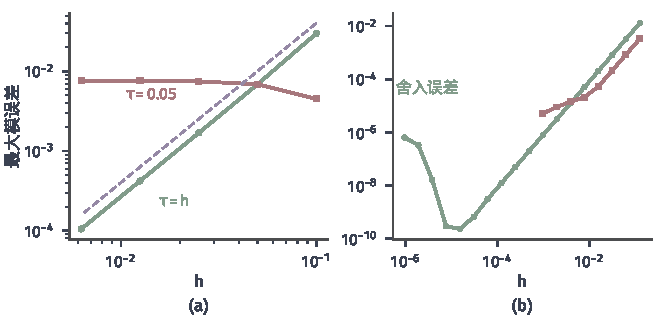
\includegraphics[width=112mm]{figures/06-differential-equations/02-partial-differential-equations/matplotlib/pdenum-error-plateau/figure.pdf}
 \caption{误差的停滞，紫色虚线是斜率$2$。(a)Crank--Nicolson方法解$u_0=\sin(\pi x)$的热方程到$T=0.1$：绿线$\tau=h$，红线固定$\tau=0.05$，后者被时间误差挡住。(b)一维Poisson问题：绿线用三对角消元直接求解，$h<2^{-16}$后舍入误差占主导；红线用共轭梯度法解$-u''=(3x+x^2)\mathrm{e}^x$，相对残差到$10^{-2}$就停止，加密后误差不再按$h^2$下降。}
 \label{fig:pdenum-error-plateau}
\end{BookInlineFigure}

积分误差也要单独看。第~\ref{sec:pdenum-assembly}小节中，同一个分片线性有限元，精确积分时节点误差为零，梯形积分时节点误差是$0.0530$，这份差别完全来自载荷的计算。

代数误差分两种。图~\ref{fig:pdenum-error-plateau}(b)的绿线是舍入误差：$\bm{A}_h$的条件数按$h^{-2}$增长，$h$小于$2^{-16}$后误差反而回升，最小值约为$2\times10^{-10}$。红线是迭代提前停止的误差：停止准则只控制残差，残差除以$\bm{A}_h$才是解的误差，所以固定的相对残差不能随网格加密自动提高解的精度。

一个实用的原则是让各段误差大致同一量级，多花的算力才有回报。迭代的容差应该随$h$收紧，时间步应该按格式的阶数跟着$h$减小。

\paragraph{计算成本}
设空间维数为$d$，每个方向的步长为$h$，未知量个数$N\sim h^{-d}$。差分和低阶有限元的矩阵每行只有常数个非零元，存储是$O(N)$。表~\ref{tab:pdenum-cost}比较了几种做法在单次求解或推进到固定时刻时的主要代价。

\begin{BookInlineTable}
 \centering
 \caption{$N\sim h^{-d}$个未知量时的代表性成本，$T$固定，常数和对数因子未写出。}
 \label{tab:pdenum-cost}
 \begin{tabular}{p{32mm}p{28mm}p{36mm}}
  \toprule
  做法 & 主要运算量 & 限制因素\\
  \midrule
  一维三对角消元 & $O(N)$ & 无\\
  带状消元，$d=2$ & $O(N^{2})$ & 带内填充，存储$O(N^{3/2})$\\
  共轭梯度，不预条件 & 约$O(N/h)$ & 迭代数随$\kappa^{1/2}\sim h^{-1}$增长\\
  显式扩散，$\tau\sim h^2$ & $O(N/h^2)$ & 稳定性\\
  隐式扩散，$\tau\sim h$ & $O(1/h)$次线性求解 & 每步的求解成本\\
  显式守恒格式，$\tau\sim h$ & $O(N/h)$ & CFL条件\\
  \bottomrule
 \end{tabular}
\end{BookInlineTable}

显式和隐式的取舍随问题而变。扩散问题的稳定性要求$\tau\sim h^2$，网格加密时显式方法的步数增长得很快，隐式方法每步更贵，但步数少得多。双曲问题的时间尺度本来就是$h$量级，显式格式的步长限制几乎不造成浪费，隐式方法反而难以获益。

大规模线性方程组的求解不在本章展开，可参考\BookChapterRef{chap:krylov-methods}{卷二第15章“Krylov子空间法”}；非线性问题每步的Newton迭代可参考\BookChapterRef{chap:second-order-methods}{卷五第7章“二阶方法”}。这些内层迭代的容差都属于式~\eqref{eq:pdenum-error-split}的最后一段。

还要记住，这些成本比较都建立在解的光滑性假设上。有激波或奇性时，全局加密的效率很低，图~\ref{fig:pdenum-fem-rates}(b)的加密网格只增加了靠近奇点的分辨率，就把一阶收敛恢复了回来。

\section{本章小结}
\label{sec:pdenum-summary}

开头的问题是：怎样把连续的场换成有限个数，这些数又代表什么。三种方法给出了三种回答，它们分别保留了连续问题的不同结构，表~\ref{tab:pdenum-methods}作了对比。

\begin{BookInlineTable}
 \centering
 \caption{三种离散方法的对比。}
 \label{tab:pdenum-methods}
 \begin{tabular}{p{16mm}p{20mm}p{20mm}p{38mm}}
  \toprule
  方法 & 未知量 & 保留的结构 & 精度保证依赖\\
  \midrule
  有限差分 & 节点值 & 局部导数 & 解的光滑性，离散逆算子的界\\
  Galerkin有限元 & 基函数系数 & 弱形式 & 有界、强制、协调，解的正则性，网格质量\\
  守恒有限体积 & 单元平均 & 局部守恒 & 守恒、相容，熵选择，全变差控制\\
  \bottomrule
 \end{tabular}
\end{BookInlineTable}

有限差分用Taylor展开逼近导数。定理~\ref{thm:pdenum-fd-error}说明，$u\in C^4$时小的截断误差经由与$h$无关的$\lVert\bm{A}_h^{-1}\rVert_\infty$转成小的解误差；解不够光滑时，阶数会下降。扩散问题上，网格加密带来更快的衰减模式，稳定性和精度对时间步提出了不同的要求。

Galerkin方法把弱问题限制到有限维子空间。Céa估计把误差化成最佳逼近问题，只用到有界性、强制性和协调性。非齐次Dirichlet数据要作提升，右端的边界贡献不能丢；实际的收敛阶还要结合解的正则性、单元次数和网格质量。

有限体积方法用界面通量更新单元平均，内部通量抵消保证了离散守恒，也保证了激波速度的正确。但守恒只管总量：Roe型通量相容又守恒，却会保留违反熵条件的膨胀激波，需要单调性或熵不等式来选出正确的解。

收敛的论证在线性和非线性问题上走了不同的路。线性格式由一致性和稳定性得到收敛，Lax等价定理说明两者在适定问题上等价；Fourier分析只适用于规则网格、常系数和周期边界，边界闭合要另行检查；CFL条件是依赖区域的必要条件，并不充分。非线性守恒格式则分别核验紧性、Lax--Wendroff定理的弱解极限和离散熵不等式，不能套用线性的结论。

因此，得到一个离散解只是开始。要说明它代表了什么连续解，还需要把空间、时间、积分和代数误差分开检验，用网格加密观察实际的收敛阶，并确认解的尺度已被网格分辨。

